\documentclass[preprint2,tighten]{aastex62}
\pdfoutput=1 %for arXiv submission
\usepackage{amsmath,amstext}
\usepackage[T1]{fontenc}
\usepackage{txfonts} %use times font for math
\usepackage[figure,figure*]{hypcap} %Figure refs go figures
\usepackage{bm}

\renewcommand*{\sectionautorefname}{Section} %for \autoref
\renewcommand*{\subsectionautorefname}{Section} %for \autoref

\newcommand*{\kms}{\,km~s$^{-1}$}
\newcommand{\todo}[1]{{\bf \textcolor{red}{ #1}}}

\shorttitle{}
\shortauthors{the IQ (Isolated \& Quenched) collaboratory}

\begin{document}


\title{Paper I: The Main Sequence of Simulated Galaxies}
%\title{Distributions of star-forming galaxies: predictions}
\author{ChangHoon Hahn}
\affil{NYU, LBL}
\altaffiliation{changhoonhahn@lbl.gov}
\author{Tjitske K. Starkenburg}
\affil{Flatiron Institute, 162 Fifth Avenue, 10010 New York, USA}
\author{Claire Dickey}
\affil{Yale University}

\author{IQ collaboratory (in alphabetical order)}
\affil{various}

\begin{abstract}


\end{abstract}
\keywords{Galaxy: halo --- Galaxy: structure}

\section{Introduction}
Generic statement about how galaxy surveys revolutionized the field and allowed
us to study the evolution of galaxy populations. The key things we learned is the
over all decline of star formation in star-forming galaxies and the rapid 
transformation of star-forming galaxies into quiescent galaxies through the 
quenching of star formation. This consequently makes understanding star-forming 
galaxies and more generally the star formation history of galaxies critical in 
galaxy evolution. 

\todo{chang: @tjitske could I assign the following paragraph to you?}
Some brief intro about the evolution of simulations. Talk about the difference 
classes of simulations: hydro sims and SAMs. The history of their attempts to 
reproduce the observed galaxy samples and how they incorporate all this nice 
physics to do so. 

This paper is the first in a series studying the star formation and quenching properties of galaxies. The series is initialized by the IQ (Isolated \& Quenched) Collaboratory. This first paper will focus on the rate of star formation in observed and simulated galaxies. Subsequent papers will build mock observational spectra for all simulated galaxies in our sample and compare spectral star formation and quenching indicators (Starkenburg et al. in prep.).

In observations the star forming galaxies are observed to lie on a tight sequence
known as the star formation main sequence. Go through the history of observations.
Measuring and understanding this sequence is important in improving our
understanding of galaxy evolution. There is however not one unified way to fit and describe the SFMS, and depending on both the dataset and the fitting technique used its properties can vary \citep[see e.g.][]{speagle2014}, adding to the complexity of the discussion on its meaning.

Nonetheless, with the key role that starforming galaxies play in our understanding of the formation and evolution of galaxies, the SFMS is an important relation to compare to for simulations. Moreover, the SFMS can form a tool to understand the starforming and non-starforming galaxy populations and the processes that create those. Therefore we argue that a comparing the galaxy populations in the SFR-$M_{\star}$ plane between different simulations that vary in technique and in descriptions of key physical processes, is important. The SFMS serves as a key feature in galaxy sample data for comparison. Therefore in this paper we compare different simulations by conducting a data-driven comparison centered around the star formation main 
sequences of different data sets. 

In Section~\ref{sec:ourgals}, we describe the simulated and observed galaxies 
used in our analysis. 


%%%%%%%%%%%%%%%%%%%%%%%%%%%%%%%%%%%%%%%%%%
% Figure 1 
%%%%%%%%%%%%%%%%%%%%%%%%%%%%%%%%%%%%%%%%%%
\begin{figure*}
\begin{center}
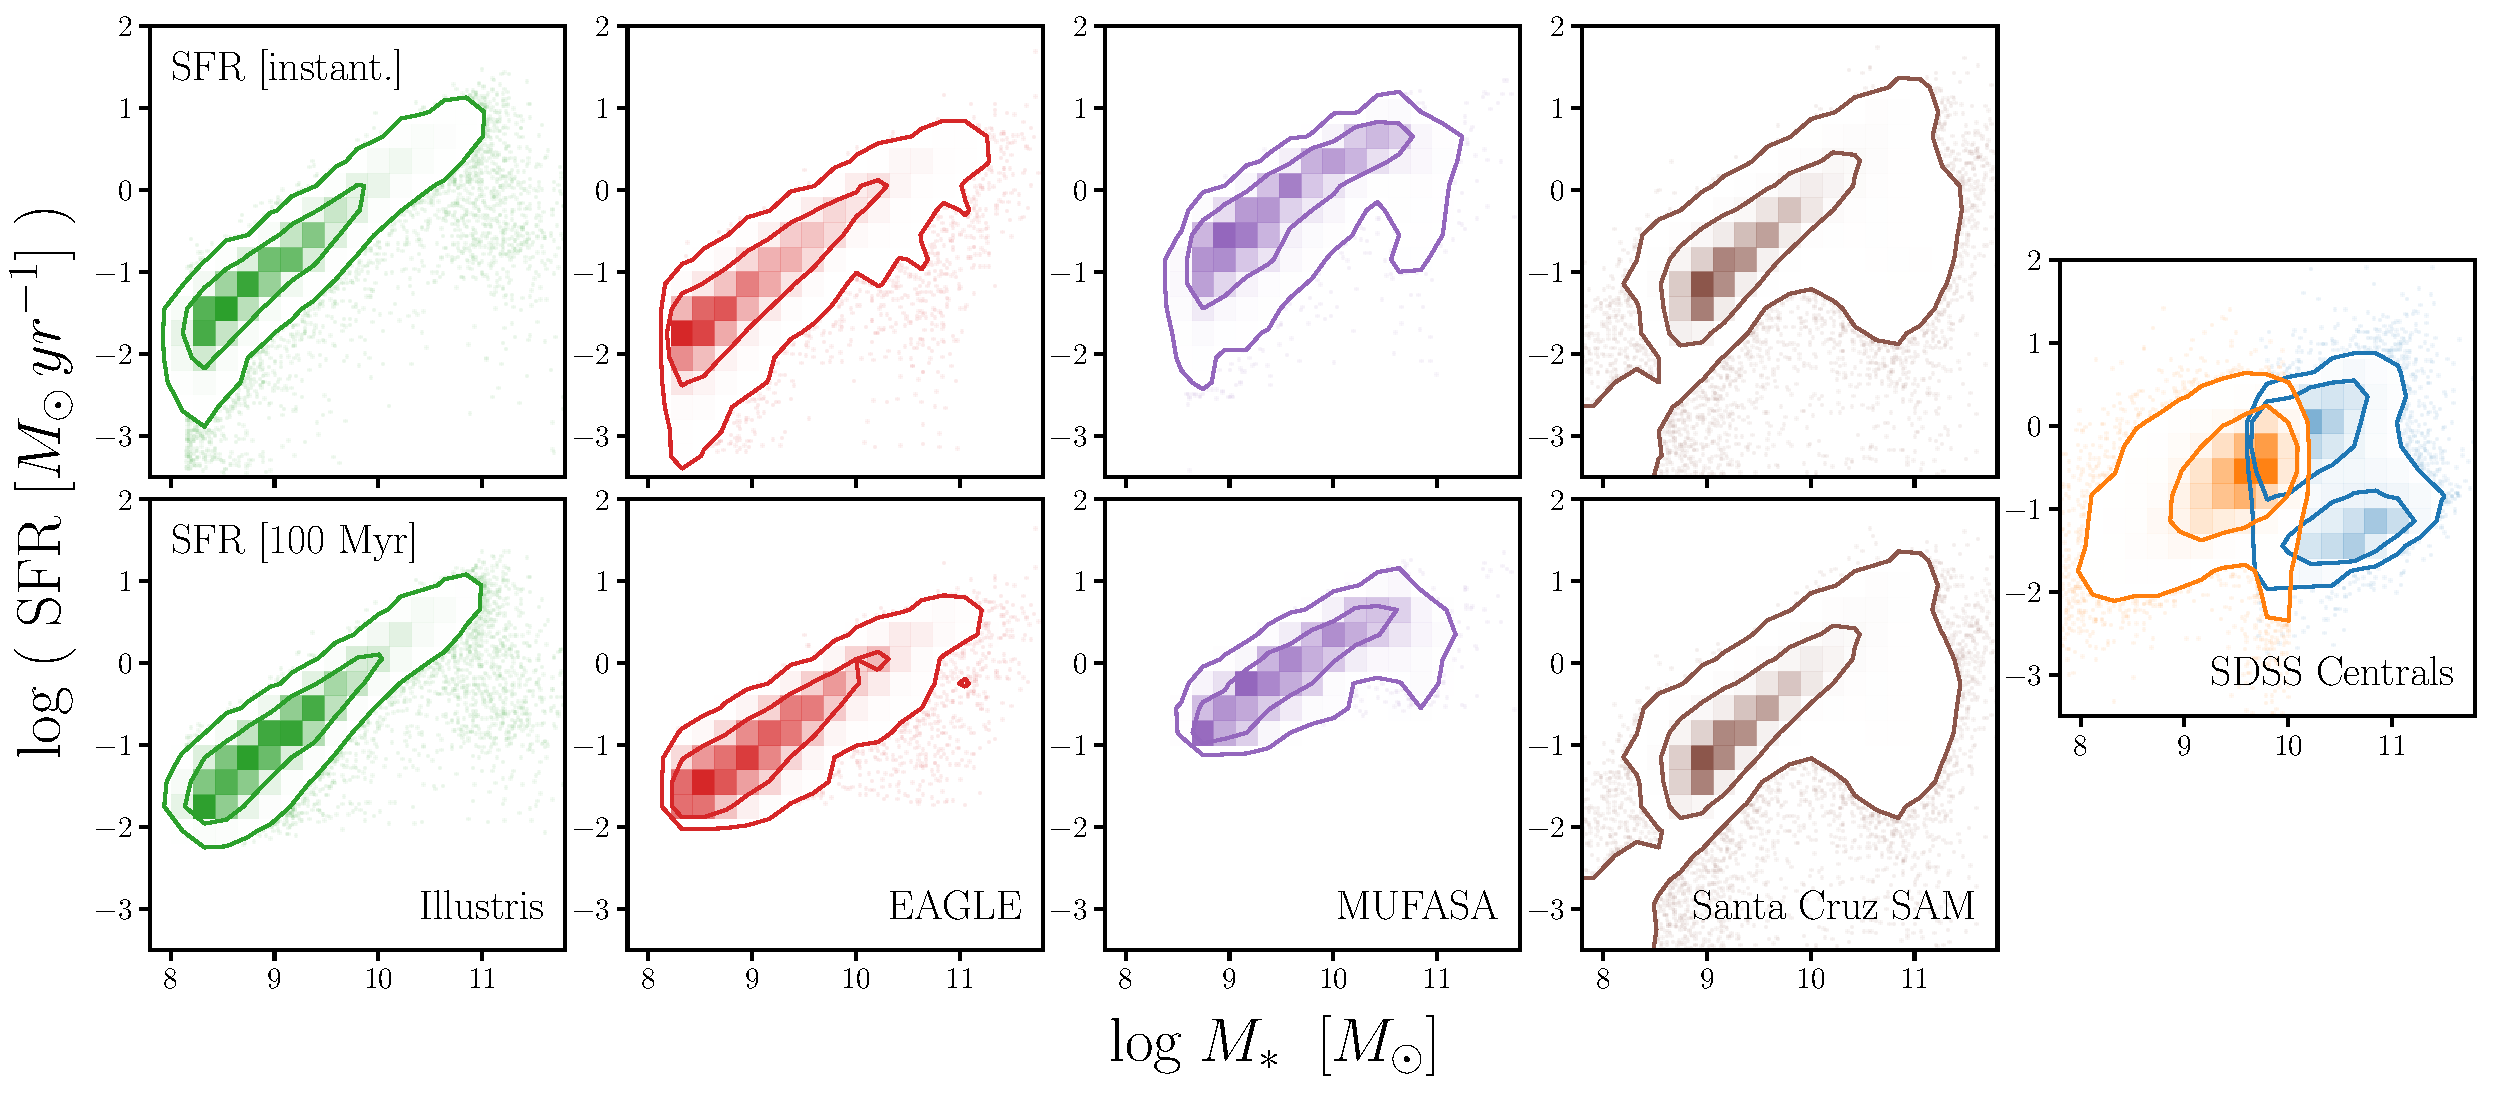
\includegraphics[width=\textwidth]{figs/Catalogs_SFR_Mstar.pdf} 
\caption{The SFR--$M_*$ relations of central galaxies from the Illustris, 
EAGLE, MUFASA, and Santa Cruz SAM simulations (left to right). The 
top panels use instantaneous SFRs while the bottom panels use SFRs 
averaged over $100\,\mathrm{Myr}$. The simulations and how they derive 
the SFRs are described in Section~\ref{sec:galsims}. Although a
direct comparison to observations is tenuous due to the fact that 
the SFRs and $M_*$s of the observed SDSS galaxies are \emph{not} 
derived consistently as simulations, we include, for reference, the 
observed  SDSS galaxies (Section~\ref{sec:obvs}) on the right. 
\emph{The $\mathrm{SFR}--M_*$ relations in every panel reveals a 
clear star forming main sequence.}} 
\label{fig:sfrmstar}
\end{center}
\end{figure*}
%%%%%%%%%%%%%%%%%%%%%%%%%%%%%%%%%%%%%%%%%%

%%%%%%%%%%%%%%%%%%%%%%%%%%%%%%%%%%%%%%%%%%
% Figure  
%%%%%%%%%%%%%%%%%%%%%%%%%%%%%%%%%%%%%%%%%%
\begin{figure}
\begin{center}
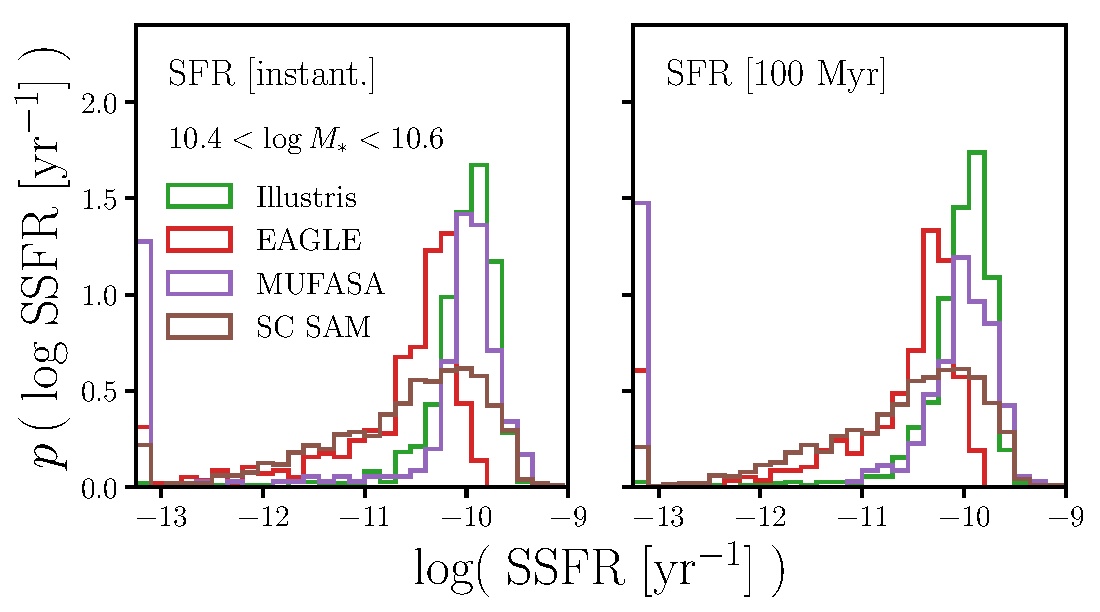
\includegraphics[width=0.475\textwidth]{figs/Catalogs_pSSFR.pdf} 
\caption{The SSFR distributions, $p(\log\,\mathrm{SSFR})$, of the 
central galaxies in the Illustris (green), 
EAGLE (red),  MUFASA (purple), and  Santa Cruz SAM (brown) simulations 
with $10.4 < \log\,M_* < 10.6$. We use instantaneous SFRs on the left
and SFRs averaged over $100\,\mathrm{Myr}$ on the right. Although the
SFMS is universal in the SFR-$M_*$ relations (Figure~\ref{fig:sfrmstar}), 
\emph{the significant discrepancies among the $p(\log\,\mathrm{SSFR})$s,
and thus SFR--$M_*$ relations, make the SFMS difficult to consistently 
quantify.} \todo{this figure is not described in the text (?)}} \label{fig:pssfr}
\end{center}
\end{figure}
%%%%%%%%%%%%%%%%%%%%%%%%%%%%%%%%%%%%%%%%%%

\section{Our galaxies} \label{sec:ourgals}
In this work, we primarily focus on galaxies in four simulated galaxy 
samples from three hydrodynamic (Illustris, EAGLE, and MUFASA) and one 
semi-analytic (Santa-Cruz SAM) large-scale cosmological simulations. 
Although we mainly restrict ourselves to simulated galaxy samples, for 
reference, we also include in our analysis two observed galaxy samples: 
a volume-limited sample from the Sloan Digital Sky Survey (hereafter SDSS) 
and a selected isolated dwarf galaxy sample from the NASA-Sloan Atlas 
(hereafter NSA). In this section, we give a brief description of the 
simulations of our data set in Section~\ref{sec:galsims}. We also briefly
describe our observed galaxy sample in Section~\ref{sec:obvs}. 
\todo{revisit once intro is written for fluidity.}

\subsection{Simulated Galaxies} \label{sec:galsims}
\todo{What are the main goals of these simulations -- i.e. what main observables are they trying to reproduce? Also, what are the main ways in which they differ from one another?}
For high-mass galaxies, the AGN-feedback descriptions in the simulations are crucial to get the right stellar--to--halo mass and color distributions. 
For lower mass systems, the stellar feedback is a very important factor for similar reasons. In all cases, the implementation of the sub-grid physics governing these feedback effects are, to a lesser or greater degree constrained by the simulation (by?) matching galaxy properties and(with?) galaxy scaling relations in the present day. Nevertheless, for both feedback prescriptions, there are a number of different (sub-grid) methods in use that will give different results on the number and properties of different galaxy populations in the SFR--$M_{\star}$ plane. 

We compare the population of the SFR--$M_{\star}$ plane between the different large-scale cosmological simulations and the observational datasets. To ensure that we compare similar star formation rate timescales, we use averaged star formation rates over different recent timescales for(from?) all the simulations. Star formation rates derived from $H{\alpha}$ observations correspond to young stars with ages $\lesssim 10\,\mathrm{Myr}$, while star formation rates derived from $UV$ brightness correspond to stars formed in the last $\sim 100\,\mathrm{Myr}$ \citep[e.g.][]{kennicutt2012}. 

Star formation rates for galaxies in our simulations can be defined on 
a range of timescales. For our analysis, however, we use SFRs averaged 
over $100\,\mathrm{Myr}$ and instantaneous SFR. \todo{motivate our choice.}
Averaged SFRs are derived using the ages of stars in the simulated 
galaxies \todo{also in the SAM? More details needed}. Meanwhile, instantaneous SFR is based on 
the rate of star formation in the dense gas of simulated galaxies. 
We note that the spatial and temporal resolution of our hydrodynamic 
simulation can significantly impact the averaged SFRs we derive for our 
simulated galaxies. In Appendix~\ref{app:zerosfr}, we discuss how we treat
resolution effects in our analysis. 

Below we give a short description of the Illustris, EAGLE, MUFASA, and 
Santa-Cruz SAM simulations, their key feedback prescriptions, and how 
we derive the instantaneous and $100\,\mathrm{Myr}$ aveaged SFRs for 
each simulation.

%For the galaxies in the simulations, we compare star formation rates averaged over the last $10\,\mathrm{Myr}$, $100\,\mathrm{Myr}$, and $1\,\mathrm{Gyr}$, as well as the instantaneous SFR. 
%We note that spatial and temporal resolution effects in the simulations  can cause averaged SFRs from stellar ages to under-predict the actual  averaged SFRs in simulations. 
%(most notably the $10\,\mathrm{Myr}$--averaged SFR) can strongly under-predict the actual averaged SFR in the simulations. We therefore add conservative upper limits and uncertainties to these values and study the effect of these on our results.

%Our figures will mostly focus on comparisons of the observationally most relevant timescales (instantaneous, $10\,\mathrm{Myr}$ and $100\,\mathrm{Myr}$) but we will comment on deviations for longer or shorter timescales.


\subsubsection{The Illustris simulation}
The Illustris simulation \citep{Vogelsbergeretal2014, Geneletal2014} evolves a cosmological volume of $(106\ \rm{Mpc})^3$ with a uniform baryonic mass resolution of $1.6\times10^6M_{\sun}$ using the Arepo moving-mesh code. The full halo mass range in the simulation is $2 \times 10^8$--$3\times 10^{14}\ M_{\sun}$, set by resolution (32 particles) at the low-mass end, and by volume (e.g.~including 10 halos with $M>10^{14}M_{\sun}$) at the high-mass end. It employs sub-grid models \citep{Vogelsbergeretal2013} for star-formation \citep{SpringelHernquist2003} and Bondi-like SMBH accretion, a phenomenological model for galactic winds, and two main modes for energy injection from SMBHs. When the accretion occurs at Eddington ratios >0.05, thermal energy is injected continuously in the local environment of the SMBH, while at lower accretion rates, the energy injection occurs in bursts at large distances from the SMBH, generating hot bubbles in the ICM \citep{Sijackietal2007}. The latter mode of feedback is responsible for a steep drop in the cosmic star-formation rate density at late times \citep{Vogelsbergeretal2013}. Previous works discussing aspects of the star-formation main-sequence and/or quenching in the Illustris simulation include \citet{Vogelsbergeretal2014, Sparreetal2015, Blucketal2016, Terrazasetal2017}.

\subsubsection{EAGLE}
The Virgo Consortium's Evolution and Assembly of GaLaxies and their Environment (EAGLE) project \citep{schaye2015, crain2015} exists of a suite of cosmological, hydrodynamical simulations of a standard $\Lambda$ cold dark matter universe using a modified version of the N-body/SPH-code Gadget 3 \citep[lastly described in][]{springel2005} called ANARCHY (Dalla Vecchia et al. in prep. see also Appendix A of \citealp{schaye2015} and \citealp{schaller2015}). Modifications include the SPH formulation, the time stepping, and the subgrid physics. The subgrid model for feedback from massive stars and AGN is based on thermal energy injection in the ISM without the need to turn-off cooling or hydrodynamic decoupling of winds \citep{dallavecchia2012}. Similarly to semi-analytical models the subgrid parameters for stellar feedback and BH accretion are calibrated based on present-day galaxy stellar mass function while also requiring reasonable galaxy sizes, and the AGN feedback efficiency is constrained by the amplitude of the central black hole-galaxy mass relation. The galaxy stellar mass range resolved is $10^{8} < M_{\star}/M_{\sun} \lesssim 10^{11}$ and the galaxy stellar mass function is reproduced to $\lesssim 0.2$ dex over this full range. The volume used in this project, L0100Ref, is has a baryonic mass resolution of $1.81\times 10^6M_{\sun}$ and a volume of $100$ cMpc on a side. In addition to the Reference version in different size boxes the EAGLE simulations suite also include higher resolution zoomed-in volumes and physics variations. The star formation--stellar mass plane and/or passive fractions in the EAGLE simulations have been previously discussed in \citet{furlong2015, trayford2015, trayford2016, trayford2017}


\subsubsection{MUFASA \todo{[Romeel]}}

\subsubsection{the Santa-Cruz Semi-Analytic Model \todo{[Rachel, Viraj]}}

\subsection{Observed SDSS Galaxies \todo{[Claire]}} \label{sec:obvs}
Our main focus in this work is to compare galaxies from our simulation. 
However, since the ultimate goal of the simulations are to reproduce 
observations, we include in our analysis galaxies from the 
SDSS volume-limited sample and the NSA low-luminosity galaxy sample. 
We provide a brief description of the two observed galaxy samples 
below. 

For the SDSS sample, we follow the sample selection of \citet{Tinkeretal2011}. 
We construct the SDSS volume-limited galaxy sample with $M_r - 5\log(h) < -18$ 
from the NYU Value-Added Galaxy Catalog \citep[VAGC;][]{Blantonetal2005} which 
corresponds to the SDSS Data Release 7~\citep[DR7;][]{Abazajianetal2009} at 
redshift $z \approx 0.04$. 
\todo{needs more details: stellar mass range}

At lower stellar masses, we use galaxies from the NSA catalog. Briefly, 
the NSA catalog is a reprocessing of SDSS DR8, optimized for low-luminosity 
objects. It relies on the improved background subtraction technique of 
\cite{blanton2011}. The catalog extends to $z \approx 0.055$ and includes 
re-calibrated spectroscopy (\todo{Yan \& Blanton 2012, Yan 2011}) with much
smaller errors. However, this recalibration is mostly relevant only at small 
equivalent width values and hence galaxies on the star formation main 
sequence will be largely unaffected by this.

For both galaxy samples, the stellar masses are estimated using the 
\citet{BlantonRoweis2007} $\mathtt{kcorrect}$ code, which assumes a 
\citep{Chabrier2003} IMF. The SFRs are derived from the SSFRs of the 
current release of 
\citet{Brinchmannetal2004catalog}\footnote{http://www.mpa-garching.mpg.de/SDSS/DR7/}. 
In \citet{Brinchmannetal2004catalog}, SSFRs 
$\gtrsim 10^{-11} \mathrm{yr}^{-1}$ are  derived from $\mathrm{H}\alpha$ 
emissions, $10^{-11}\gtrsim$ SSFRs $\gtrsim 10^{-12} \mathrm{yr}^{-1}$ 
are derived from a combination of emission lines, and SSFRs 
$\lesssim 10^{-12} \mathrm{yr}^{-1}$ are mainly based on $D_n4000$. 
We emphasize that SSFRs $\lesssim 10^{-12} \mathrm{yr}^{-1}$ should only be 
considered upper limits to the true value \citep{Salimetal2007}.

%%%%%%%%%%%%%%%%%%%%%%%%%%%%%%%%%%%%%%%%%%%%%%%%%%%%
% Section 
%%%%%%%%%%%%%%%%%%%%%%%%%%%%%%%%%%%%%%%%%%%%%%%%%%%%
\subsection{Identifying Isolated/Central Galaxies}
We're interested in \todo{something consistent with the intro}. \todo{discuss the halo finder and effect on central/satellite}
However, it's well established that galaxies in their detailed properties
carry the imprint of their environment (~\citealp{hubble1936, oemler1974, dressler1980, balogh}, for a recent review see ~\citealp{blanton2009}). 
In addition to the dependence of the quiescent fraction on 
environment~\citep[\emph{e.g.}][\todo{more citations}]{peng2010,hahn2015}, the different 
timescales of star formation quenching in central versus satellite 
galaxies~\citep{wetzel2013,hahn2017a} suggest that different physical 
mechanisms impact galaxy star formation in different environments. 
Furthermore,~\cite{wang2018} recently 
found significant discrepancies between the SFMSs of central versus 
satellite galaxies. In order to remove the impact of galaxy environment
in our analysis, we focus only on central galaxies, which constitute 
over $70\%$ of $M_* > 10^{9.7}M_\odot$ galaxies at $z=0$. 

Despite the long recognized importance of galaxy environment, centrals 
are often heterogeneously defined in the 
literature~\citep[see][]{campbell2015}. Centrals in our 
simulations (see Section~\ref{sec:galsims}) are similarly classified 
inconsistently \todo{(something about how the halos are different and 
that propagates to central classifications. maybe a sentence on what they do?)} 
Furthermore, the underlying dark matter information is used for the 
classification. Such a classification, which cannot be reproduced on 
observed galaxy samples, complicate comparison to observations.
Therefore, we identify central galaxies in all of our simulations 
consistently using an extended version of the~\cite{tinker2011} group 
finder, designed to identify satellite/centrals in observations. 

\begin{itemize}
\item description of Jeremy's new group finder code along with 
\item some discussion on the discrepancy between what the simulations consider central and what the group finder considers centrals 
\end{itemize}
\emph{Galaxies with $P_\mathrm{sat} < 0.01$ are designated as centrals.} 

Overall, we find good agreement between the central classifications of 
the group finder and simulations. Using purity and completeness as defined 
in Eqs.~13 and~15 of~\cite{campbell2015}, we find purities of 
$99\%, 93\%, 84\%$, and $90\%$ and completenesses of $86\%$, $89\%$, 
$91\%$, and $86\%$  for the Illustris, EAGLE, MUFASA and Santa Cruz SAM 
simulations respectively. For the hydrodynamic simulations, we find no 
significant stellar mass dependence in the purities. However, the Santa 
Cruz SAM has purity of $44\%$ at $M_*$ below $10^{8.5}M_\odot$ and $97\%$ 
above. Consequently, we impose a stellar mass limit of $M_* > 10^{8.5} M_\odot$
for the Santa Cruz SAM. In addition to the overall agreement in central 
classifications, we confirm that the group finder classification does \emph{not} 
impact the results of this paper. Next, using the identified central 
galaxies from our simulations, we proceed to fitting the star formation 
main sequence in the next section.

%To define isolated galaxies we employ different methods to the volume limited datasets and the large cosmological simulations, and to the SDSS-NSA dataset and the zoom simulations. In all cases the simulated galaxies are treated in a similar sense as the observed galaxies, and a probability of being a satellite is derived for all galaxies.

%%%%%%%%%%%%%%%%%%%%%%%%%%%%%%%%%%%%%%%%%%
% Figure 
%%%%%%%%%%%%%%%%%%%%%%%%%%%%%%%%%%%%%%%%%%
\begin{figure*}
\begin{center}
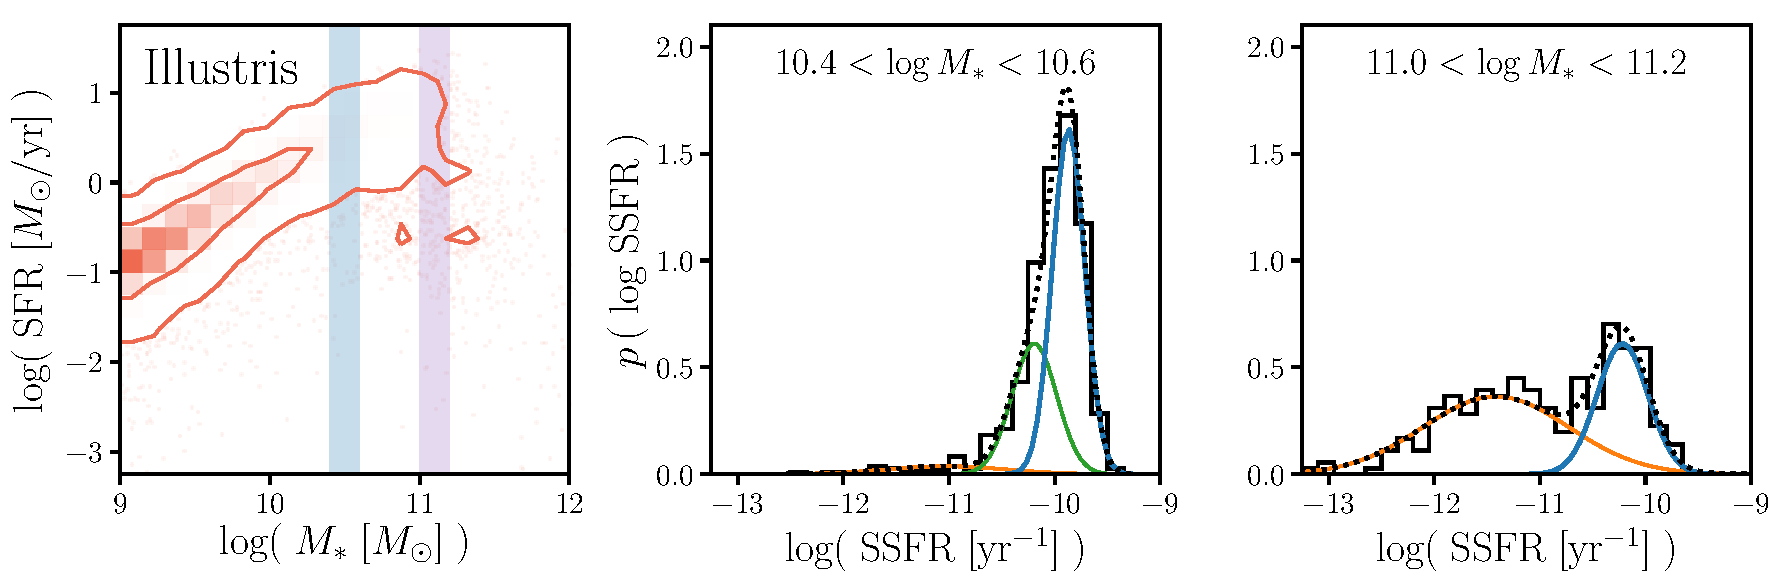
\includegraphics[width = 0.9\textwidth]{figs/SFMSfit_demo.pdf} 
\caption{
Our GMM SFMS fitting method for Illustris central galaxies in two 
stellar mass bins: $10.4 < \log\,M_* < 10.6$ (\emph{center}) and 
$11.0 < \log\,M_* < 11.2$ (\emph{right}), highlighted on the SFR--$M_*$ 
relation (\emph{left}). On the right, we compare the SSFR 
distributions, $p(\log\,\mathrm{SSFR})$, in the two stellar 
mass bins to their best-fit GMMs of our SFMS fitting method. The 
$p(\log\,\mathrm{SSFR})$ in the center panel is best described by a 
GMM with three components (orange, green, and blue) while the
$p(\log\,\mathrm{SSFR})$ in the right panel is best described by 
a GMM with two components (orange and blue). The SFMS components of the 
best-fit GMMs are plotted in blue. \emph{Our SFMS fitting can identify the 
SFMS for a wide variety of SSFR distributions without hard assumptions or 
cuts to the sample.}
}\label{fig:fitdemo}
\end{center}
\end{figure*}
%%%%%%%%%%%%%%%%%%%%%%%%%%%%%%%%%%%%%%%%%%

\section{Fitting the Star Formation Main Sequence}\label{sec:sfmsfit}
From the SFR-$M_*$ relations of our central galaxies obtained from the simulations and 
SDSS observations of Section~\ref{sec:ourgals}, which we present in 
Figure~\ref{fig:sfrmstar}, we note the following: regardless of the SFR 
timescale (top/bottom) or simulation and over four orders of magnitude 
in stellar mass, \emph{the SFR and $M_*$ of star-forming galaxies are 
tightly correlated}. In fact, observations have long established this 
so-called \emph{star formation main sequence} (hereafter SFMS) beyond the 
local universe out to 
$z > 2$~\citep[\emph{e.g.}][\todo{more}]{noeske2007,salim2007}. 
Besides its persistence in observations and simulations, as highlighted 
earlier, the SFMS describes the star-forming population and hence plays
a crucial role in understanding galaxy evolution. A key step then is to 
robustly and consistently identify the SFMS in data. 

Although the SFMS is universal among a wide range of observations
and simulations, different datasets give rise to significantly different 
star formation--stellar mass distributions. This makes the SFMS difficult 
to \emph{consistently} quantify. So far in the literature, a wide variety 
of fitting methods have been applied to data. For instance, \cite{bluck2016} 
fit the SFMS using median $\log\mathrm{SFR}$s of galaxies with 
$M_* < 10^{10}M_\odot$ and extrapolate to higher $M_*$s. This method, however, 
assumes that all $M_* < 10^{10}M_\odot$ galaxies lie on the SFMS and that 
the slope of the SFMS is constant throughout the stellar mass range of the 
data. Alternatively, \cite{lee2015} fit the SFMS using median 
$\log\,\mathrm{SFR}$s of galaxies in the sample after some color-color cut 
to identify SF galaxies. Other recent works in the literature have opted 
for more sophisticated methods such as fitting a three-component
Gaussian~\citep{bisigello2018} or a zero-inflated negative binomial 
distribution~\citep{feldmann2017}. 

Despite their variety, many of these methods require arbitrary assumptions 
or hard cuts on the sample. Moreover, as we find, it's challenging to use 
these methods to fit the SFMS over the wide SFR and $M_*$ ranges we're 
interested in for the different simulations and observations. In an effort 
to better fit a wide variety of star formation--stellar mass distributions 
and relax the assumptions and cuts imposed on the data, we present a flexible 
and data-driven method for fitting the SFMS that makes use of Gaussian Mixture 
Density Estimation~\citep[GMMs;][]{Press:1992:NRC:148286, 9780471006268}. 
Besides its comprehensive use in machine learning and statistics, Gaussian 
Mixture Density Estimation has also been used in wide range of astronomical 
analyses~\citep{hogg2010,bovy2011,lee2012,taylor2015}.



\subsection{Using Gaussian Mixture Models}
Gaussian Mixture Density Estimation uses a Gaussian Mixture Model 
(hereafter GMM), a weighted sum of $k$ Gaussian component densities 
\begin{equation} \label{eq:gmm}
\hat{p}(x;\bm{\theta}) = \sum\limits_{i=1}^{k} \pi_i \, \mathcal{N}(x; \bm{\theta}_i),
\end{equation}
to estimate the density. The weights, $\pi_i$, mean, and variance  
$\bm{\theta}_i=\{\mu_i, \sigma_i\}$ 
of the components are free parameters in the GMM. For a given data set 
$\{x_1, ..., x_n\}$, these parameters are most commonly estimated through
the expectation-maximization algorithm~\citep[EM;]{dempster1977,neal1998}. 
Starting with randomly assigned $\bm{\theta}_{i}^0$ to the $k$ GMM components, 
the EM algorithm iterates between two steps. First, for every data point, 
$x_i$, the algorithm computes for a probability of $x_i$ being generated by 
each GMM component. These probabilities act as assignment weights to each of
the components. Next, based on these weights, $\bm{\theta}_i^t$ of the components 
are updated to $\bm{\theta}_i^{t+1}$ to maximize the likelihood of the assigned 
data. $\pi_i$ are also updated by summing up the assignment weights and 
normalizing the sum by the total number of data points. These steps are 
repeated until convergence --- \emph{i.e.} when $p(\{x_1, ..., x_n\} ; \bm{\theta}_t)$ 
converges. Instead of starting with randomly assigning $\bm{\theta}_{i}^0$, 
we initiate our EM algorithm using a $k$-means clustering algorithm~\citep{lloyd1982}.
More specifically, for our Gaussian mixture density estimation we use 
the $k$-$\mathtt{means}$++ algorithm of~\cite{arthur2007}. 

For our actual SFMS fitting method, we begin by dividing the galaxy 
sample into stellar mass bins of specified $\Delta \log\,M∗$ width. In 
this paper we use bins of $\Delta \log\,M∗ = 0.2\  \mathrm{dex}$; however, 
this choice does not significantly impact the final fit. For each stellar 
mass bin, if there are more than $N_\mathrm{thresh}=100$ galaxies in the bin, 
we fit the SSFR distribution using Gaussian mixture models (GMMs) 
with 1 to 3 components with parameters determined from the EM algorithm 
described above. Our restriction to models with a maximum of 3 components 
is motivated by the three possible galaxy classifications: quiescent, 
star-forming, and transitioning populations. \todo{insert sentence about the $k > 3$ test.}
Out of the three GMMs, we 
select the ``best-fit'' model with the lowest Bayesian Information 
Criteria~\citep[BIC;][]{schwarz1978}. BIC is often used in conjunction with 
GMMs~\citep[\emph{e.g.}][]{leroux1992,roeder1997,fraley1998,steele2010performance} 
and also more generally for model selection in 
astronomy~\citep[\emph{e.g.}][]{liddle2007,broderick2011,vakili2016}.
In addition to the likelihood, BIC introduces a penalty term for the number
of parameters in the model. This way, using BIC not only finds a good fit to 
the data, but it also addresses the concern of over-fitting. 
% CHH: not sure if we want to include this figure}.
% In Figure~\ref{fig:gmm_pedagog},  

In the best-fit GMM, we designate the Gaussian component of the 
best-fit GMM with mean $\log\,\mathrm{SSFR} > −11$ as the SFMS component.
In the case when more than one GMM component has mean 
$\log\,\mathrm{SSFR} > −11$, the component with the larger weight 
(\emph{i.e.} the mode) is designated as the SFMS component. In such a 
situation, the SFRs of the SFMS is not well described by a log-normal
distribution. In observations (Section~\ref{sec:obvs}), we do not 
encounter this situation in any of the stellar mass bins. In simulations, 
however, we encounter this situation in lower stellar mass bins 
($\log\,M_* < 10^{9}\ M_\odot$) of the Illustris and EAGLE simulations. 

In Figure~\ref{fig:fitdemo}, we plot the best-fit GMM for the 
central galaxies of the Illustris simulation in two stellar mass 
ranges highlighted in the left panel: $10.4 < \log\,M_* < 10.6$ (center) 
and $11.0 < \log\,M_* < 11.2$ (right). For the two stellar mass bins, 
we compare the SSFR distributions of the bins to the components of the 
best-fit GMMs derived from our SFMS fitting method. The SFMS component 
is plotted in blue. The SSFR distribution of the center panel is best 
described by a GMM with three components while the SSFR distribution 
in the right  panel is best described by a GMM with only two components.
The right panels illustrate the wide variation in SSFR distributions of 
the galaxy samples. More importantly, it highlights the effectiveness 
of our fitting method in identifying the SFMS for different SSFR 
distributions. All the code used for our SFMS fitting is publicly available 
at \url{https://github.com/changhoonhahn/LetsTalkAboutQuench}.

\todo{So far we have assumed that one, two, or three populations would describe galaxies in the SFR--$M_*$ plane well. We have checked whether the possibility of adding more than three Gaussians in the GMM shows that more populations are present. This is the case only for the Santa Cruz semi-analytic model, where in a number of bins the presence of 4, 5, or (in one case) 6 Gaussians is preferred. In almost all cases the added Gaussians have low weight and form effectively additional intermediate populations. For both Illustris and EAGLE there is only one mass bin where a fourth population would be preferred. For all other mass bins in all the hydrodynamical simulations, and all mass bins in the SDSS 3 or less Gaussians are preferred.}
%%%%%%%%%%%%%%%%%%%%%%%%%%%%%%%%%%%%%%%%%%
% Figure
%%%%%%%%%%%%%%%%%%%%%%%%%%%%%%%%%%%%%%%%%%
\begin{figure*}
\begin{center}
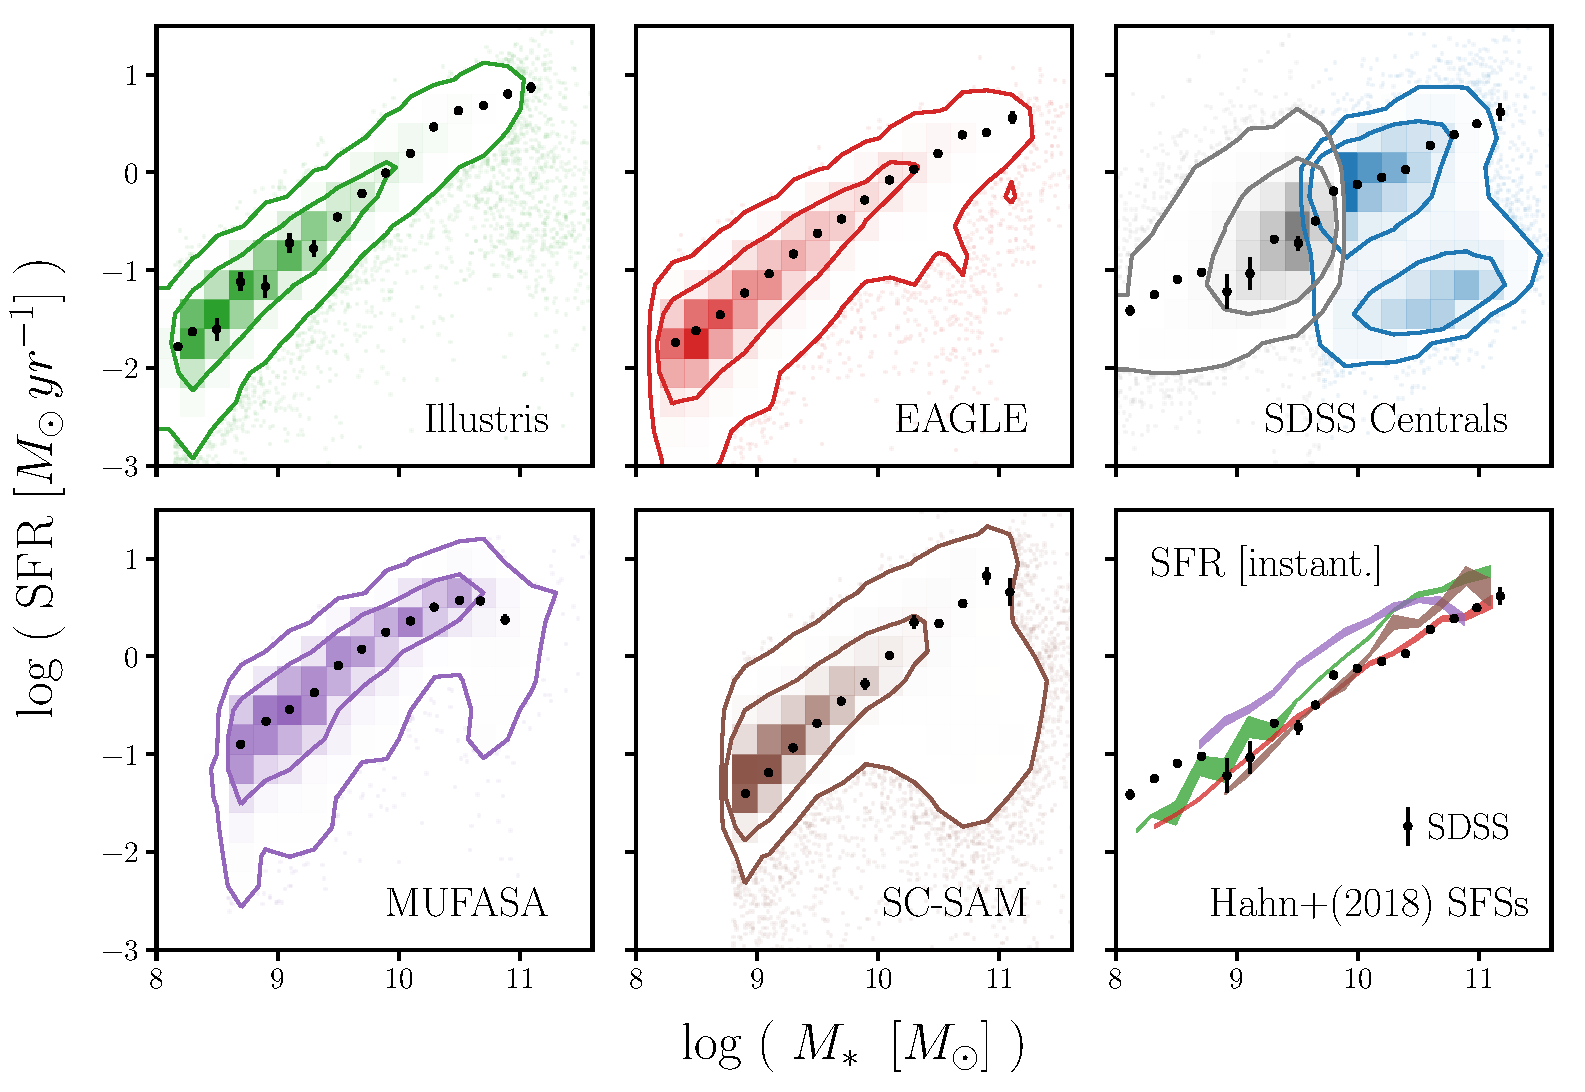
\includegraphics[width = 0.8\textwidth]{figs/Catalogs_SFMSfit_SFRinst.pdf} 
\caption{Best-fit SFMS of the central galaxies in the Illustris, EAGLE, MUFASA, 
and Santa Cruz SAM simulations as identified by our SFMS fitting method 
(Section~\ref{sec:sfmsfit}). The SFMSs above are fit from the instantaneous 
SFR to $M_*$ relation. We compare the SFMS fits to one another in the bottom 
right panel. For reference, we include the best-fit SFMS of the SDSS sample 
in the top right panel. \emph{The SFMSs of the simulations have similar 
slopes -- i.e. stellar mass dependence. Their amplitude, however, roughly 
vary by an order of magnitude.}} \label{fig:sfmsfit_inst}
\end{center}
\end{figure*}
%%%%%%%%%%%%%%%%%%%%%%%%%%%%%%%%%%%%%%%%%%

%%%%%%%%%%%%%%%%%%%%%%%%%%%%%%%%%%%%%%%%%%
% Figure  
%%%%%%%%%%%%%%%%%%%%%%%%%%%%%%%%%%%%%%%%%%
\begin{figure*}
\begin{center}
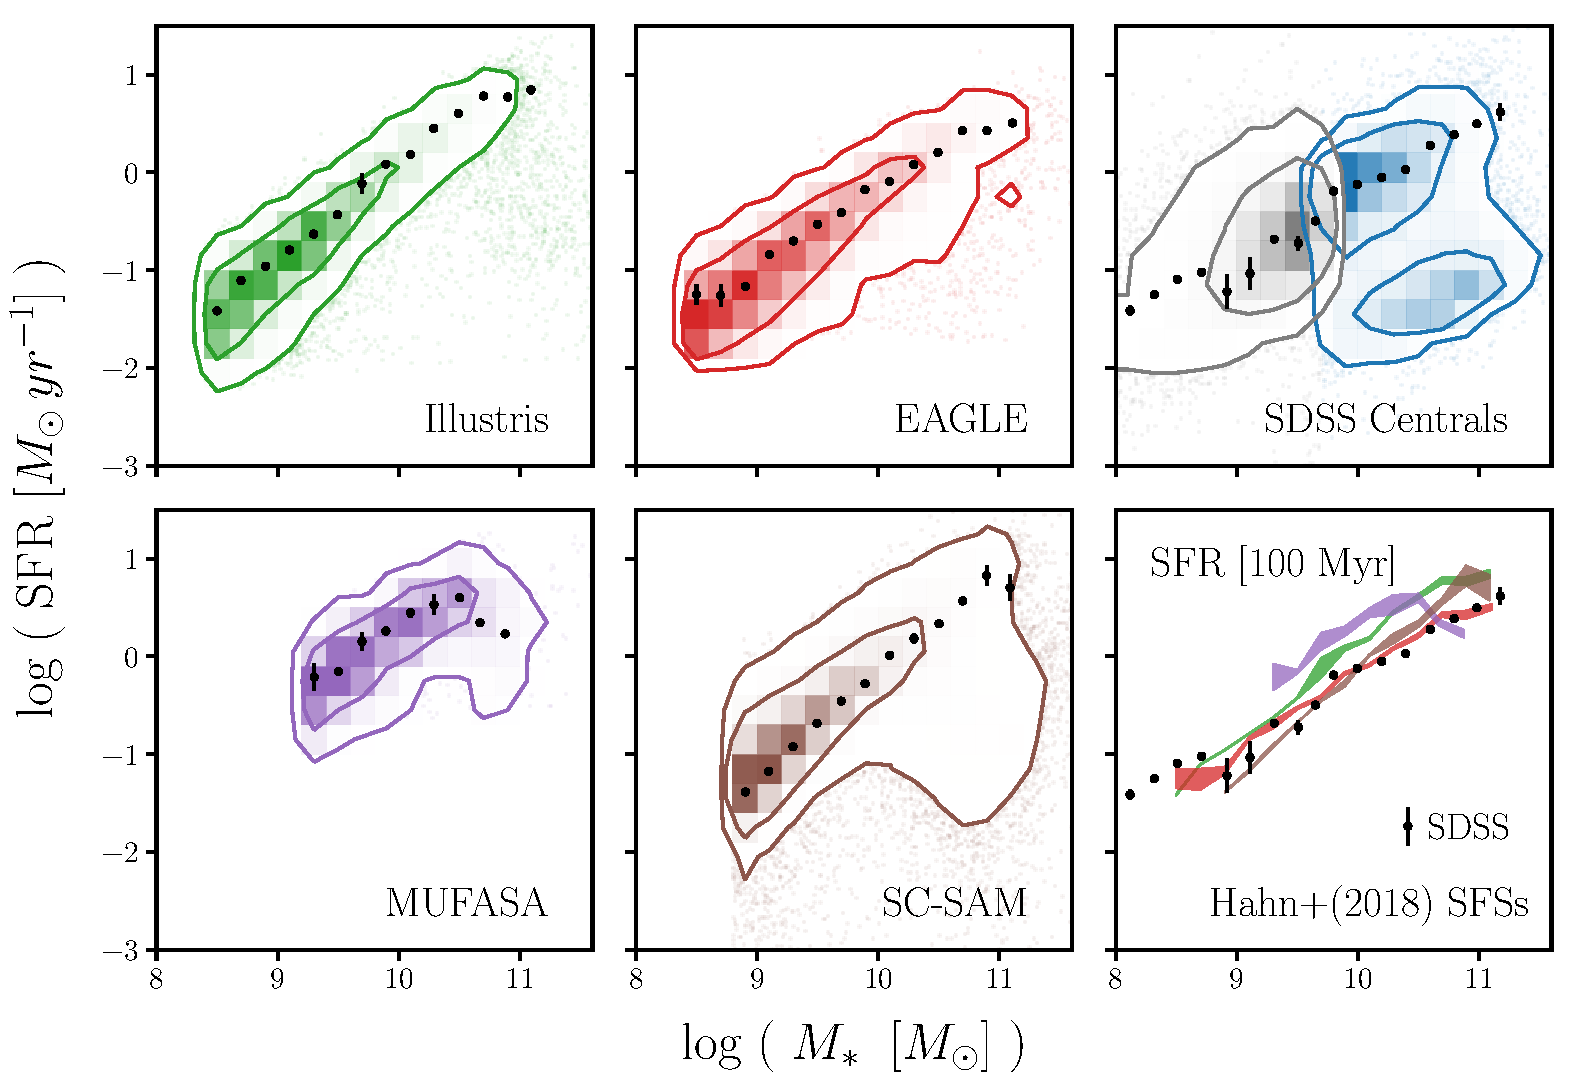
\includegraphics[width = 0.8\textwidth]{figs/Catalogs_SFMSfit_SFR100myr.pdf} 
\caption{Same as Figure~\ref{fig:sfmsfit_inst} but for the SFR-$M_*$ relation 
using SFR averaged over $100\,\mathrm{Myr}$. As in   
Figure~\ref{fig:sfmsfit_inst}, \emph{the SFMSs of the simulations have similar 
slopes but vary roughly by an order of magnitude in amplitude.}}
\label{fig:sfmsfit_100myr}
\end{center}
\end{figure*}
%%%%%%%%%%%%%%%%%%%%%%%%%%%%%%%%%%%%%%%%%%

%%%%%%%%%%%%%%%%%%%%%%%%%%%%%%%%%%%%%%%%%%
% Figure  
%%%%%%%%%%%%%%%%%%%%%%%%%%%%%%%%%%%%%%%%%%
\begin{figure}
\begin{center}
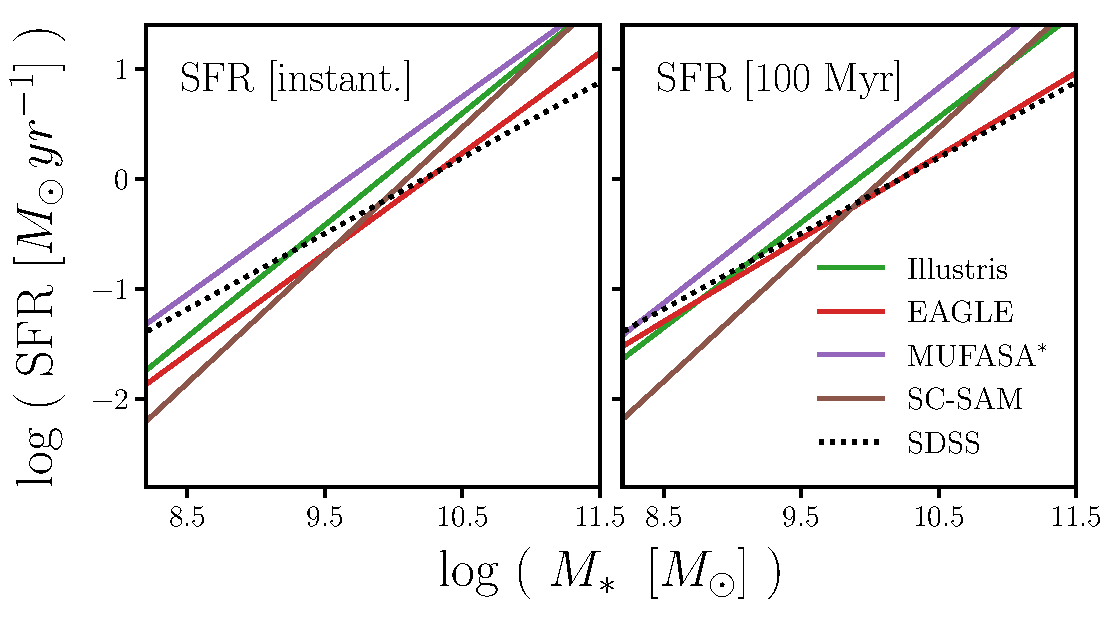
\includegraphics[width = 0.5\textwidth]{figs/Catalogs_SFMS_powerlawfit.pdf} 
\caption{Power-law fits to the best-fit SFMS from our GMM fitting method 
for the Illustris (green), EAGLE (red), MUFASA (purple), and Santa Cruz 
SAM (brown) simulations. The left and right panels use instantaneous SFR 
and $100\,\mathrm{Myr}$ SFR, respectively. We list the the power-law fit
parameters in Table~\ref{tab:sfms_powerlaw}. Aside from the MUFASA power-law
fit which is affected by the high stellar mass turnover, we find no significant
mass dependence in the discrepancies among the power-law fits. Throughout 
the stellar mass range, the Illustris, EAGLE, and Santa Cruz SAM SFMS power-law 
fits differ by $\sim 0.5\mathrm{dex}$. 
}\label{fig:sfmsfit_powerlaw}
\end{center}
\end{figure}
%%%%%%%%%%%%%%%%%%%%%%%%%%%%%%%%%%%%%%%%%%

\section{Results} \label{sec:results}
\subsection{SFMS of simulated galaxies}
Now that we have a method for fitting the SFMS (Section~\ref{sec:sfmsfit}), 
which flexibly applies to a wide range of SSFR distributions 
(Figure~\ref{fig:fitdemo}), we can identify the SFMSs of our simulated
central galaxies from Section~\ref{sec:ourgals}. For the two SFR timescales,
instantaneous and $100\,\mathrm{Myr}$, we present the best-fit SFMSs of our 
simulated galaxies from the Illustris, EAGLE, MUFASA, and Santa Cruz SAM 
simulations in Figures~\ref{fig:sfmsfit_inst} and~\ref{fig:sfmsfit_100myr}, 
respectively. %For reference we include the best-fit SFMS of the SDSS central galaxies in the top right panel. 

Besides identifying the SFMSs for each of the simulations, the best-fit
SFMSs also allow us to make detailed comparison among the simulations. 
Aside from MUFASA, the best-fit SFMSs of the simulations exhibit a similar
monotonic relation between SFR and $M_*$ out to $M_* \sim 10^{11}M_\odot$, for 
all SFR timescales. The best-fit SFMSs for MUFASA, however, turn over at 
$M_* \sim 10^{10.5} M_\odot$ and decreases in SFR at high stellar masses. 
We confirm that this turnover is \emph{not} caused by misidentification of 
the SFMS or some systematic effect of the fitting by examining the GMM 
components of the best-fit and the $p(\mathrm{SSFR})$ in these higher 
stellar mass bins. When we compare the best-fit SFMSs of the simulations 
altogether in more detail, we find \emph{order of magnitude discrepancies 
in SFR among the best-fits throughout the stellar mass range of the 
simulations for both SFR timescales} (bottom right panels of 
Figures~\ref{fig:sfmsfit_inst} and~\ref{fig:sfmsfit_100myr}). 

From the best-fit SFMSs identified for our galaxies, we can further 
parameterize the SFMS to some functional form as often done in the 
literature --- \emph{e.g.} power-law~\citep{speagle2014} or broken 
power-law~\citep{lee2015}. With little evidence of a turnover in the 
SFMS for most of our galaxies, we fit a power-law of the form 
\begin{equation} \label{eq:powerlaw}
\log\,\mathrm{SFR}_\mathrm{MS} = m\,(\log\,M_* - 10.5) + b
\end{equation}
to the SFMSs in Figure~\ref{fig:sfmsfit_powerlaw}. We list the best-fit 
(maximum likelihood) parameter values of Eq.~\ref{eq:powerlaw} in 
Table~\ref{tab:sfms_powerlaw}. The power-law parameterizations accentuate 
the stellar mass dependence of the SFMSs and can reveal the mass dependence 
in the discrepancies 
among the SFMSs. Putting aside MUFASA, which has a significant turnover at high 
stellar masses, we find significant discrepancies in the slopes of the SFMSs
of the simulations with Santa Cruz SAM having the steepest SFMS and EAGLE 
having the shallowest SFMS. The power-law SFMS fits, however, reveal little 
mass dependence in the discrepancies of the SFMSs. For instantaneous SFR, 
the discrepancies between Illustris, EAGLE, and Santa Cruz SAM are 
$\sim 0.5\,\mathrm{dex}$ throughout the stellar mass range. Meanwhile, 
for $100\,\mathrm{Myr}$ SFR, we find slightly
greater discrepancies among Illustris, EAGLE, and Santa Cruz SAM throughout
the stellar mass range.

%At lower stellar masses (), for both instantaneous SFRs and $100\,\mathrm{Myr}$ SFRs, the SFMS disagree with each  other by more than an order of magnitude. \todo{talk about how MUFASA for 100 Myr is an outlier because of the high  stellar mass limit and the high mass turnover.}
\begin{itemize}
\item \todo{What's causing the simulations to have SFMSs that are almost an 
order of magnitude different?} 
\item \todo{How come this doesn't cause cosmic star-formation rate 
density estimates to also be an order of magnitude different?}
\item \todo{what's up with MUFASA. why does MUFASA it have a turnover? -- 
mufasa's quenching is based on halo mass?}
\end{itemize}
%%%%%%%%%%%%%%%%%%%%%%%%%%%%%%%%%%%%%%%%%%
% Table
%%%%%%%%%%%%%%%%%%%%%%%%%%%%%%%%%%%%%%%%%%
\begin{table}
\caption{Power-law fit to the SFMS of our simulated central galaxies from the
Illustris, EAGLE, MUFASA, and Santa Cruz SAM simulations.\todo{update}} 
\begin{center}
\begin{tabular}{p{5cm}cc} \toprule
%\multicolumn{2}{c}{} \\[-7pt]
\multicolumn{3}{c}{Star Forming Main Sequence fit} \\
\multicolumn{3}{c}{$\log\,\mathrm{SFR}_\mathrm{MS} = m\,(\log\,M_* - 10.5) + b$  } \\ [5pt]
Simulation & $m$ & $b$ \\ 
\hline
Illustris [inst. SFR] & 0.96 & 0.51 \\ 
Illustris [$100\,\mathrm{Myr}$ SFR] & 0.96 & 0.54 \\ [2pt]
EAGLE [inst. SFR] & 0.86 & 0.17 \\ 
EAGLE [$100\,\mathrm{Myr}$ SFR] & 0.76 & 0.18 \\ [2pt]
MUFASA [inst. SFR] & 0.69 & 0.50 \\ 
MUFASA [$100\,\mathrm{Myr}$ SFR] & 0.57 & 0.44 \\ [2pt]
Santa Cruz SAM [inst. SFR] & 1.10 & 0.36 \\ 
Santa Cruz SAM [$100\,\mathrm{Myr}$ SFR] & 1.11 & 0.36 \\ 
\hline
\end{tabular} \label{tab:sfms_powerlaw}
\end{center}
\end{table}
%%%%%%%%%%%%%%%%%%%%%%%%%%%%%%%%%%%%%%%%%%

The uncertainties associated to the best-fit SFMSs in 
Figures~\ref{fig:sfmsfit_inst} and~\ref{fig:sfmsfit_100myr} 
are derived from bootstrap resampling (\todo{cite?}) in each stellar mass 
bin of the fitting. These uncertainties are \emph{underestimates} because 
they do not account for ``cosmic variance'' --- \emph{i.e.} we only have one 
finite volume realization of each simulation. Uncertainty of the best-fit 
SFMS corresponds to the uncertainty of the means of the SFMS GMM component, 
which is only one of the parameters in the GMM. Uncertainties from bootstrap 
resampling, however, do \emph{not} account for the correlations between the 
mean of the SFMS GMM and other
parameters of the GMM (Eq.~\ref{eq:gmm}). A more robust estimate of the 
uncertainties would involve estimating the marginalized posterior distribution 
of the SFMS GMM component mean using a method like MCMC. Since this still 
does not account for cosmic variance, we use bootstrap uncertainties. 

One factor that impacts our SFMS fits is the strict lower limit of the 
$\log\,\mathrm{SFR}$s, illustrated in the $100\,\mathrm{Myr}$ SFR -- 
$M_*$ relations of the hydrodynamical simulations of Figure~\ref{fig:sfrmstar} 
--- especially MUFASA. This limit is caused by resolution effects in 
the simulations, which are particularly evident at the lower mass end. 
As we describe in~\ref{sec:galsims}, the $100\,\mathrm{Myr}$ SFRs are 
calculated using \todo{chh: fill appropriate detail}. For a galaxy to 
have star formation (\emph{i.e.} SFR $> 0$), it must \emph{at least} 
form one star particle over $100\,\mathrm{Myr}$. A single star particle 
forming over $100\,\mathrm{Myr}$ amounts to a SFR of 
$\sim 0.02\ M_{\sun}\ yr^{-1}$ for Illustris and EAGLE and
$\sim 0.2\ M_{\sun}\ yr^{-1}$ for MUFASA. This resolution limit, due to 
the slope of the SFMS, ultimately impacts the 
SFMS fits at stellar masses below $10^{8.4}M_\odot$, $10^{8.6}M_\odot$, 
and $10^{9.4}M_\odot$ for 
Illustris, EAGLE, and MUFASA respectively (Appendix~\ref{app:zerosfr}). 
These stellar mass limits have accordingly been imposed on the SFMS fits
and power-law SFMS fits in Figures~\ref{fig:sfmsfit_100myr} 
and~\ref{fig:sfmsfit_powerlaw}.

\todo{concluding paragrpah to this subsection that ties together all the
results regarding the sfms}

%%%%%%%%%%%%%%%%%%%%%%%%%%%%%%%%%%%%%%%%%%
% Figure  
%%%%%%%%%%%%%%%%%%%%%%%%%%%%%%%%%%%%%%%%%%
\begin{figure}
\begin{center}
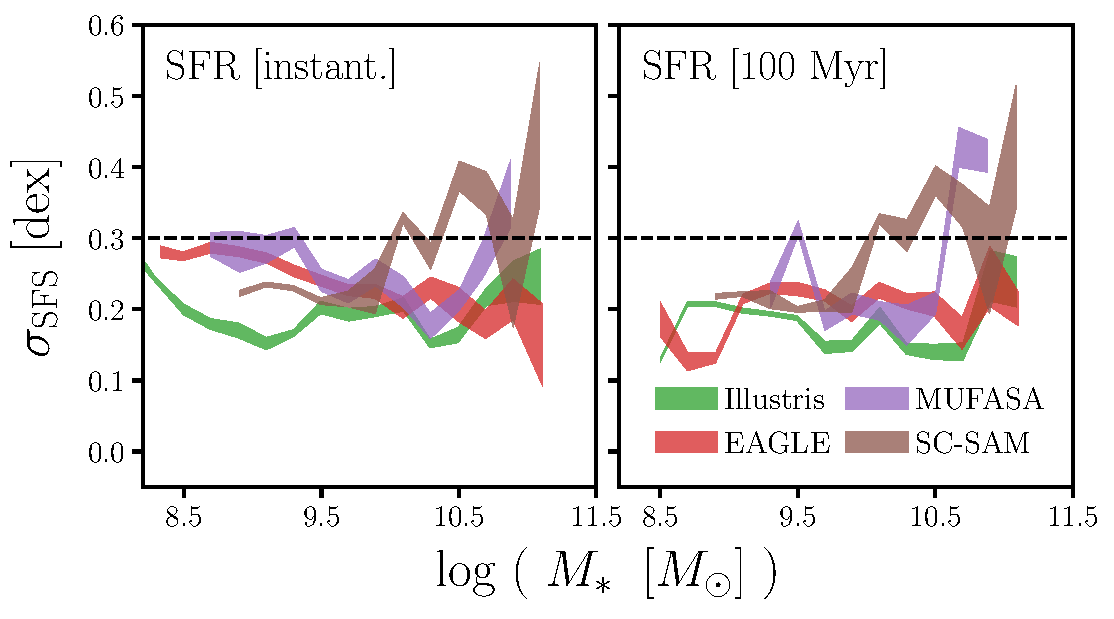
\includegraphics[width=0.48\textwidth]{figs/Catalogs_SFMS_width.pdf}
\caption{The width of the SFMS, $\sigma_\mathrm{SFMS}$, for our simulated 
central galaxies from the Illustris, EAGLE, MUFASA, and Santa Cruz SAM in 
green, red, purple, and brown respectively. The widths are derived from  
the GMM SFMS fitting and its uncertainties are estimated using bootstrap
resampling in the same way as the SFMS fit uncertainties. The
$\sigma_\mathrm{SFMS}$s in our simulations have little stellar mass 
dependence and, once measurement errors in SFR are accounted for, they 
are in agreement with the $\sim 0.3\mathrm{dex}$ observed SFMS width 
(black dashed).} \label{fig:sfms_width}
\end{center}
\end{figure}
%%%%%%%%%%%%%%%%%%%%%%%%%%%%%%%%%%%%%%%%%%


%%%%%%%%%%%%%%%%%%%%%%%%%%%%%%%%%%%%%%%%%%
% Figure  
%%%%%%%%%%%%%%%%%%%%%%%%%%%%%%%%%%%%%%%%%%
\begin{figure*}
\begin{center}
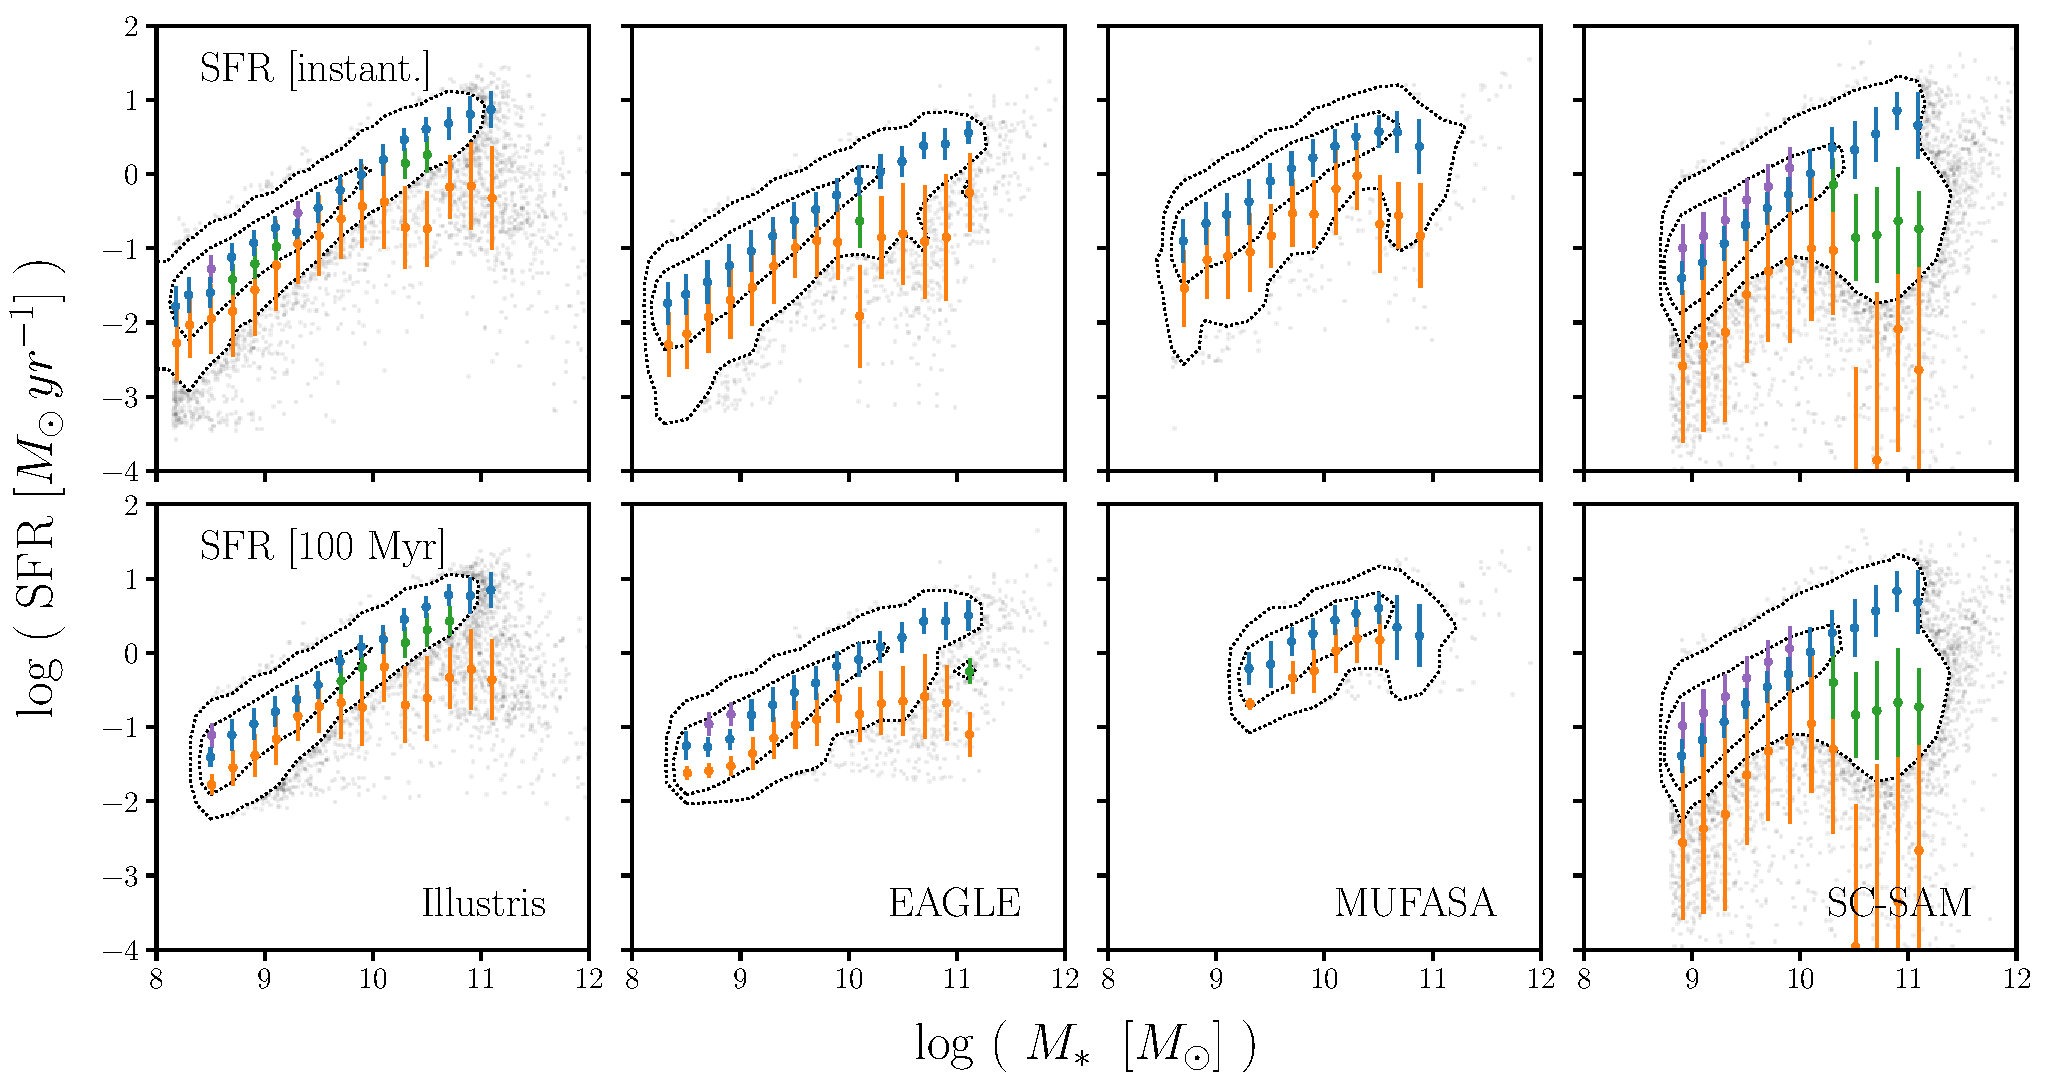
\includegraphics[width=\textwidth]{figs/Catalogs_GMMcomps.pdf} 
\caption{Components of the best-fit GMM from our SFMS fitting method for the
SFR-$M_*$ relations of central galaxies in the Illustris, EAGLE, MUFASA, and 
Santa Cruz SAM simulations (left to right). The top panels use instantaneous 
SFRs while the bottom panels use SFRs averaged over $100\,\mathrm{Myr}$. 
For reference, we also include observed centrals from SDSS (top right). We mark 
the SFMS components in blue, the components with lowest SFR in orange, 
and the other components in green. These components {\em loosely} correspond
to the star-forming, quiescent, and transitioning populations. 
Although the simulations have good agreement in their SFMSs
(Figures~\ref{fig:sfmsfit_inst}~and~\ref{fig:sfmsfit_100myr}), these GMM components
reveal the more detailed discrepancies among the simulations. 
} \label{fig:sfmsfit_comps}
\end{center}
\end{figure*}
%%%%%%%%%%%%%%%%%%%%%%%%%%%%%%%%%%%%%%%%%%


%%%%%%%%%%%%%%%%%%%%%%%%%%%%%%%%%%%%%%%%%%
% Figure 
%%%%%%%%%%%%%%%%%%%%%%%%%%%%%%%%%%%%%%%%%%
\begin{figure*}
\begin{center}
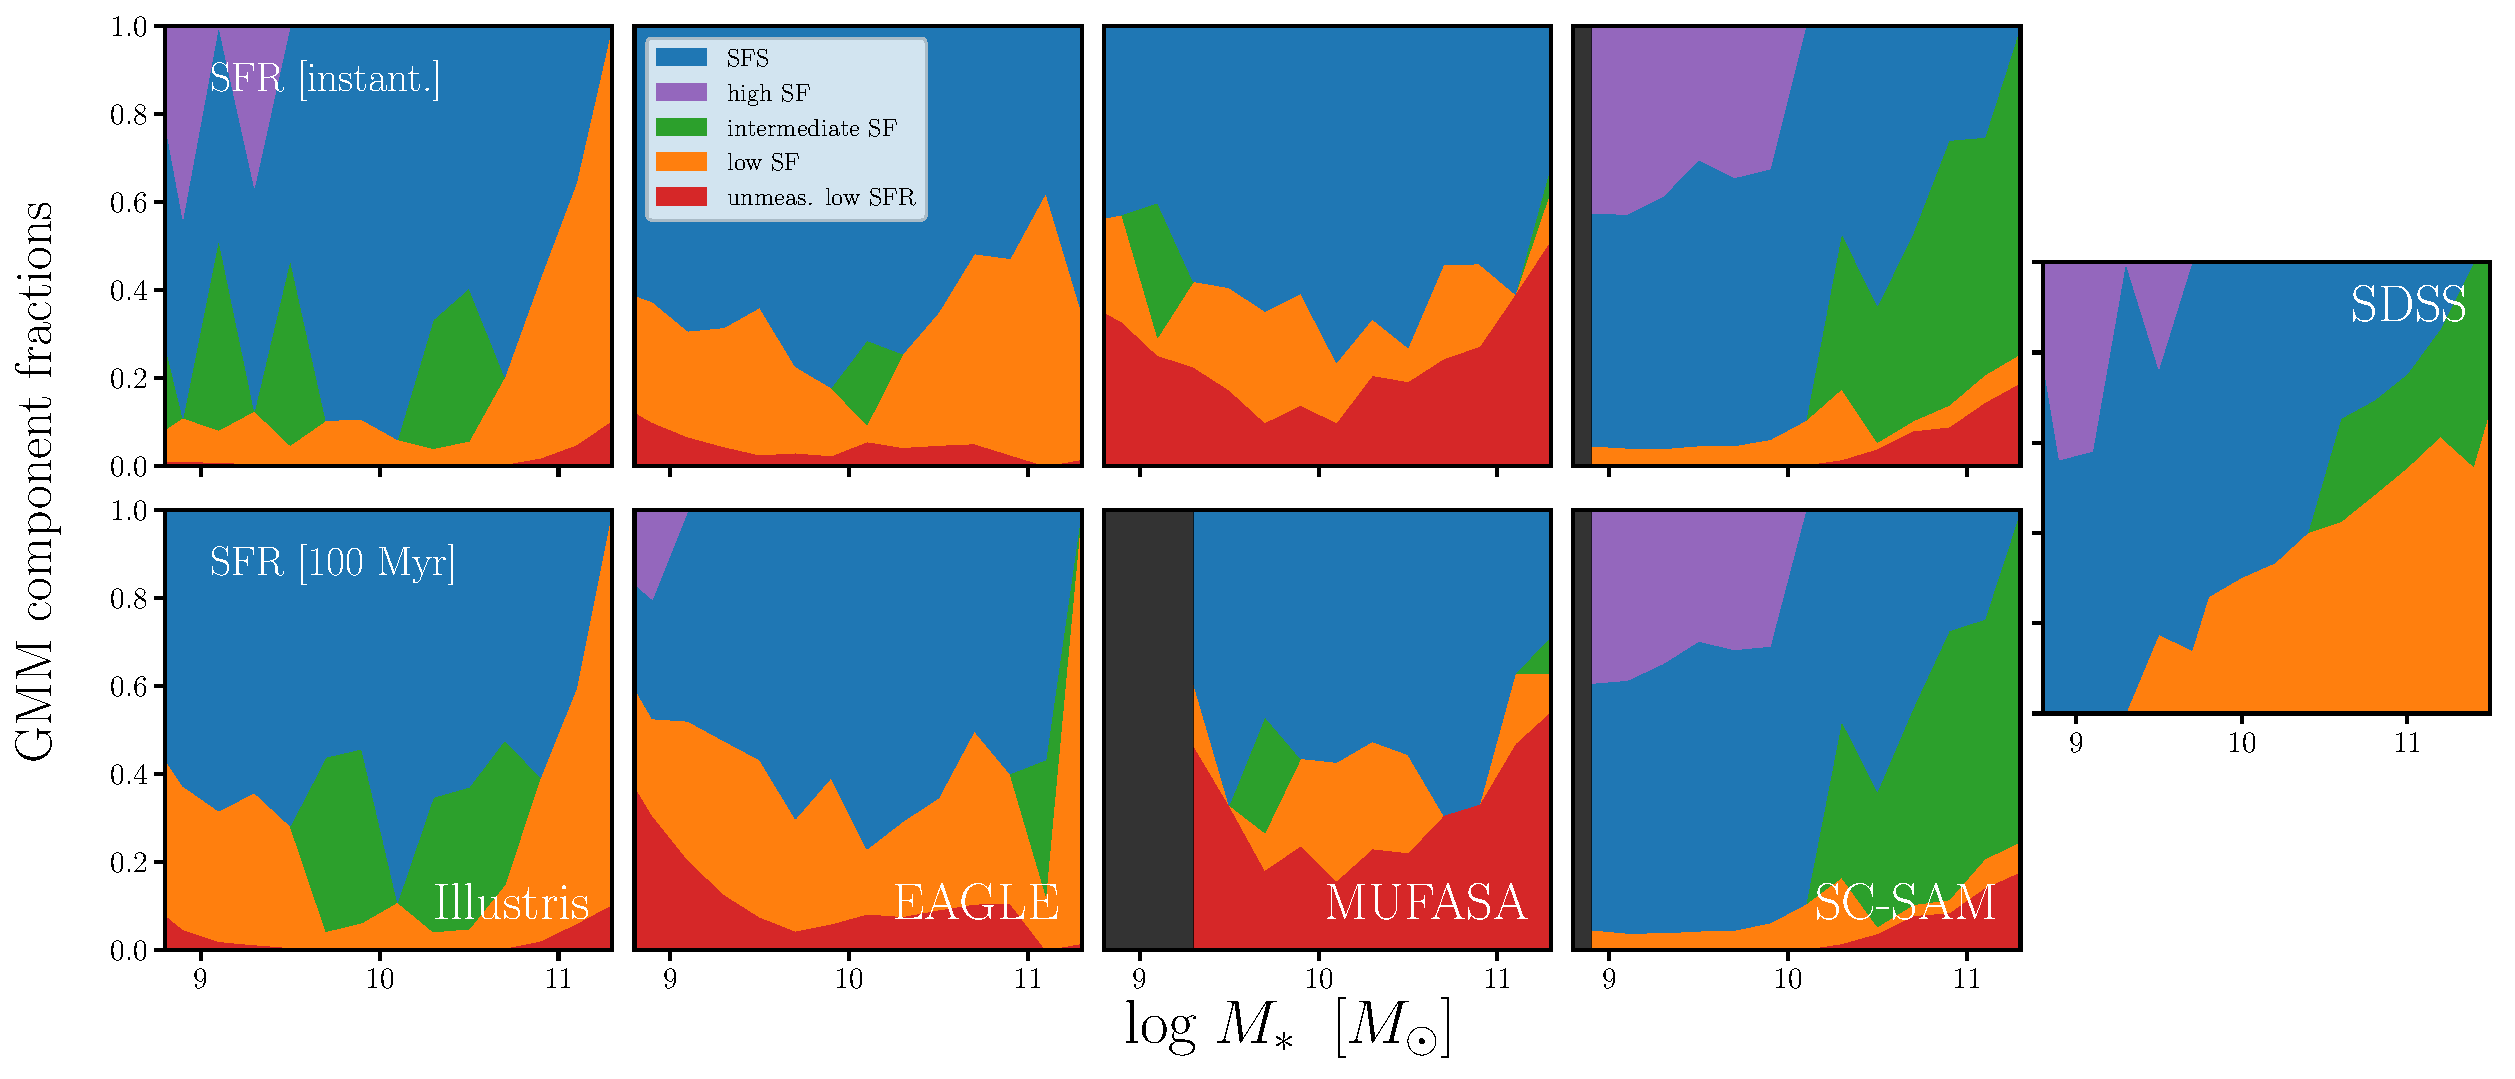
\includegraphics[width=0.9\textwidth]{figs/GMMcomp_composition.pdf} 
\caption{Fractional contributions of the best-fit GMM components from 
our SFMS fitting of the central galaxies in the Illustris, EAGLE, MUFASA, 
and Santa Cruz SAM simulations (left to right). We highlight the SFMS 
component in blue, the quenched component in orange, galaxies with 
SFR$=0$ in red, the intermediate components in green, and the star-burst
components in purple. The quenched component corresponds to \todo{finish}. 
} \label{fig:kandinsky}
\end{center}
\end{figure*}
%%%%%%%%%%%%%%%%%%%%%%%%%%%%%%%%%%%%%%%%%%

\subsection{Beyond the SFMS of simulated galaxies}
So far, we have focused solely on the position of the SFMSs for our simulated
galaxies. Our SFMS fitting method from Section~\ref{sec:sfmsfit}, however, 
also determines the width of the SFMS and identifies components other than 
the SFMS. We can therefore compare the widths of the SFMS, 
$\sigma_\mathrm{SFMS}$, as a function of $\log\,M_*$ among the simulations
in~\ref{fig:sfms_width}. The uncertainties for the widths are calculated 
through bootstrap resampling in the same way as the uncertainties for the
SFMS fits. They therefore underestimate the actual uncertainties. 
Overall, we find little stellar mass dependence in $\sigma_\mathrm{SFMS}$ 
for the simulations. For Illustris, EAGLE, MUFASA, and Santa Cruz SAM we respectively find 
$\sigma_\mathrm{SFMS} \sim 0.16, 0.20, 0.21$, and $0.20\,\mathrm{dex}$ 
for instantaneous SFR and
$\sigma_\mathrm{SFMS} \sim 0.17, 0.24, 0.23$, and $0.24\,\mathrm{dex}$
for $100\,\mathrm{Myr}$ SFR. The widths of the SFMS in the simulations 
are generally narrower than the $\sim 0.3\,\mathrm{dex}$ width measured
in observations~\citep[\emph{e.g.}][]{daddi2007, noeske2007, magdis10, whittaker12}. 
This difference, however, does not account for the uncertainties in the 
observed SFR measurements. If accounted for this would reduce the 
discrepancy. We therefore conclude that \emph{the width of the SFMS from our 
simulations are in reasonable agreement with the observed SFMS width.}

The GMM components other than the SFMS component, also offer interesting
insights into the other galaxy populations. When we examine the mean and 
variance of all the components from our fitting for our simulated galaxies 
we find interesting correspondence between the components and the quiescent,
transitioning, and star-burst galaxy populations
(Figure~\ref{fig:sfmsfit_comps}).
Similar to how we designated the SFMS component of the GMM, we 
can also designate the GMM component with the lowest SFR as the quiescent 
component, the GMM component with SFR in between the SFMS and the quiescent 
components as transitioning, and the GMM component with SFR higher than the 
SFMS component as the star-burst component. In Figure~\ref{fig:sfmsfit_comps}, 
we mark the SFMS components in blue, quiescent components in orange, and 
the other components in green. 

All of the simulations have significant populations below the SFMS at all 
masses. The hydrodynamical simulations have relatively tight quiescent components 
$\sim 1\,\mathrm{dex}$ below the SFMS. The quiescent components of the 
Santa Cruz SAM, meanwhile, are much broader and extend below 
$\log\,\mathrm{SFR} = -4$. Regardless of their position and width, the 
significant quiescent populations at low stellar masses are in disagreement
with observations~\citep{geha2012}, which find no isolated/central quenched 
galaxies below $M_* \sim 10^9 M_\odot$. 
\todo{Some sentence about what may be causing this.}
This discrepancy between simulations and observations, however, must be 
taken with a grain of salt. Both the environment and quenched classifications 
in \cite{geha2012} are defined differently than in the simulations. 
\cite{geha2012} classifies as a galaxy as quenched if it
does not have an $H\alpha$ emission and based on a $D_n 4000$ criteria. 
Furthermore, \todo{the isolation criteria of \cite{geha2012} is more 
stringent than the group finder. (CHH: @claire is this true?)} 
%incept the idea for paper2. 

Figure~\ref{fig:sfmsfit_comps} reveals components besides the SFMS and quiescent
components. For instance, in Illustris and the Santa Cruz SAM, our GMM fitting
finds a number of components between the SFMS and quiescent components ---
\emph{i.e.} transitioning galaxies. For Illustris, transitioning components 
are identified at $10^9 M_\odot < M_* < 10^{11}M_\odot$. For the Santa Cruz SAM, 
transitioning components are identified at $M_8 > 10^{10} M_\odot$. We also 
identify components with SFRs above the SFMS. These \emph{star-burst} 
components are particularly evident in the Santa Cruz SAM, where a significant
star-burst population is observed at $10^9 M_\odot < M_* < 10^{10} M_\odot$. 
Besides the Santa Cruz SAM, we also find star-burst components at the lowest
stellar masses ($M_* < 10^9 M_\odot$) of the Illustris and EAGLE simulations 
for $100\,\mathrm{Myr}$ SFRs. 

The different components we identify using the GMM fitting allows us to make a 
number of interesting comparisons of the simulated galaxies. Overall
the galaxies from hydrodynamical simulations have similar components
and features. Besides the difference in the position and width of the SFMS, 
the only significant discrepancy is the transitioning components of
Illustris. In fact the transitioning components in the Illustris galaxies 
helps explain the tighter width of the SFMS compared to the other hydrodynamical 
simulations in Figure~\ref{fig:sfms_width}. A more significant difference 
revealed by the components is the discrepancy between the hydrodynamical 
simulations and the SAM. 
\begin{itemize}
\item[-] Why is the SAM so different overall?
\item[-] Why does Santa Cruz SAM have a broader SFR? 
\item[-] Why does Santa Cruz SAM have star-bursts in "intermediate" stellar masses
\end{itemize}

Another set of parameters we infer from our GMM fitting is the weight of the 
GMM components ($\pi_i$) in Eq.~\ref{eq:gmm}. Since each of the components 
correspond to a galaxy population, these weights correspond to the fractional
contribution of the different populations. Then the fractional contribution 
of the quenched component is an estimate of the quiescent 
fraction~\citep[\emph{e.g.}][]{blanton2009, geha2012,hahn2015}. We present 
the fractional contribution of all the components from our GMM fitting as a
function of stellar mass in Figure~\ref{fig:kandinsky}: SFMS (blue), 
quenched (orange), $\mathrm{SFR}=0$ galaxies (red), intermediate (green), 
and star-burst (purple). We present the uncertainties of $\pi_i$ estimated
through bootstrap resampling in Figure~\ref{fig:fcomp_uncertainty} of 
Appendix~\ref{app:zerosfr}. 
For every simulation, a significant fraction of galaxies have SFR$=0$. 
This is because \todo{chang: @tjistke why do we have a significant fraction 
of galaxies with SFR$=0$ in all of the simulations?} 

The fractional contributions of the GMM components in Figure~\ref{fig:kandinsky}
present a number of disagreements between trends established from 
observations and our simulated galaxies --- especially the ones from 
hydrodynamical simulations. As we mentioned earlier, observations 
established a stellar mass lower bound for isolated/central quenched
galaxies. From Figure~\ref{fig:kandinsky}, we find significant quiescent
populations at $M_* < 10^9 M_\odot$, confirming the trends from 
Figure~\ref{fig:sfmsfit_comps}. Including SFR$=0$ galaxies, the quiescent 
fraction for the EAGLE simulation is roughly $0.4$ at $10^9M_\odot$. 
Illustris with $100\,\mathrm{Myr}$ SFRs and MUFASA with instantaneous SFRs
have similarly high quiescent fractions. Even in the Santa Cruz SAM, we 
find a non-negligible ($\sim 10\%$) quiescent fraction at $10^9M_\odot$. 

Related to the low $M_*$ quiescent fraction, we find little stellar mass 
dependence in the fraction of high SFR components (blue and purple) at 
$M_* < 10^{11} M_\odot$ for our hydrodynamical simulations. 

\todo{concluding paragrpah to this subsection that ties together all the
results regarding the sfms: 
highlight the advantage of our GMM fitting method
highlight how the data-driven fitting method provides detailed insights into 
simulated galaxies besides the ones that lie on the SFMSs .
We ultimately conclude from these insights that the hydro sims do not agree
well with trends established from observations. Santa Cruz SAM does better.}

\subsection{Comparing to Observations}
Our data-driven GMM SFMS fitting has so far provided a principled way to 
compare our simulated galaxy populations through the major features in the 
data. These comparisons have revealed a number of agreements and discrepancies
among the simulations; however, the ultimate goal of these galaxy simulation 
is to reproduce the observations. Therefore, in this section we compare 
our simulations to our observed galaxy sample from SDSS and NSA
(Section~\ref{sec:obvs}) in a similar fashion to the previous sections. 

First, we compare the SFMS of our simulated galaxies to the best-fit SFMS
of our SDSS and NSA central galaxies
(Figure~\ref{fig:sfmsfit_inst} and~\ref{fig:sfmsfit_100myr}). 
we find that the simulations have a steeper SFMS than our observations

Looking beyond the SFMS, 
The SDSS samples show a SFR-$M_*$ relation that is best fitted by \emph{one} Gaussian at lower masses, unlike any of the simulations. This is noteworthy even though the low-mass sample is far from volume-complete and especially many low-SFR galaxies may be missed at lower masses.
%\item[-] The observations show a very well defined, and for higher mass bins quite narrow, low-SFR population, with a small intermediate third population for only three mass bins. The low-SFR population is more narrow and generally with the mean at slightly lower SFR than for all three hydro simulations. It is located in between the intermediate and low-SFR populations of the SAM.

The comparison between our simulations and observations have been pretty 
qualitative. We deliberately refrain from a more detailed comparison due 
to the limitations of such a comparison. The SFRs and $M_*$, the main 
galaxy properties considered in this paper, are defined and measured 
differently in simulations versus observations. SFRs from the SDSS and 
NSA catalogs are measured using a combination of $H\alpha$ and $D_n 4000$. 
Although we choose the SFR timescales to best reflect observed SFRs, 
\todo{TKS: Compare to Speagle2014 combined dataset fits and discuss with respect to the large discrepancy they note in MS-slopes for the SDSS sample of $~0.4$ dex. This is partly due to using different SFR indicators (nice segue to the 2nd and 3rd papers), but not completely}
we're still comparing apples to oranges. 
In the next paper we will bring this comparison on a more equal footing 
by deriving star formation rates from mock observations of the simulated 
galaxies (Starkenburg et al. in prep.).

%comparison to observations are complicated by a number of factors.  First the SFRs and stellar masses of observations are defined by kcorrect  and emission lines and dn4000. While our SFR timescales were chosen to best  reflect the observed SFR, it's still not an apples to apples comparison.  Second, the stellar mass and SFRs of observed galaxies have uncertainties  associated to them. If unaccounted for, these uncertainties will impact the  components recovered from the GMM fitting and ultimately the SFMS fits. 
%All of the points in this subsection are severely affected by the different ways that SFR (and $M_*$) are measured in the observations and the simulations. 

\section{Summary and Conclusions} \label{sec:summary}
conclusion!

\appendix
%%%%%%%%%%%%%%%%%%%%%%%%%%%%%%%%%%%%%%%%%%
% Figure j 
%%%%%%%%%%%%%%%%%%%%%%%%%%%%%%%%%%%%%%%%%%
\begin{figure}
\begin{center}
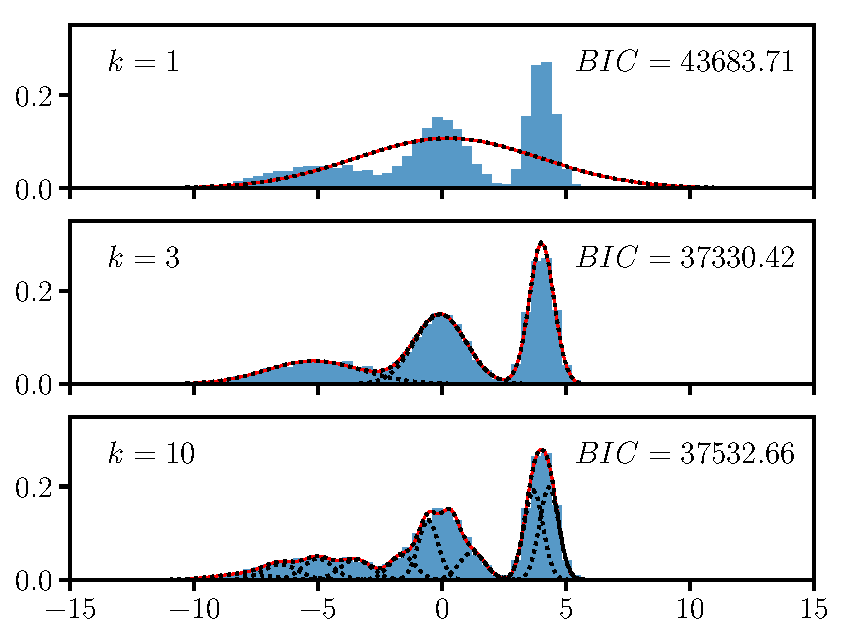
\includegraphics[width = 0.475\textwidth]{figs/GMM_pedagog.pdf} 
\caption{A pedagogical illustration of Gaussian mixture density estimation. 
We use GMMs with $k = 1$ (top), $3$ (middle), $10$ (bottom) components to estimate 
the distribution of data (blue) drawn from three Gaussian distributions. The GMM 
outputs of the EM algorithm are plotted in red with dotted lines representing each 
of their components. We also include the BIC of the GMMs, which we use to select 
the number of components $k$. Of the three panels, $k=3$ has the lowest BIC and 
therefore best represents the data according to our selection 
scheme. \todo{move to appendix}} \label{fig:gmm_pedagog}
\end{center}
\end{figure}
%%%%%%%%%%%%%%%%%%%%%%%%%%%%%%%%%%%%%%%%%%

%%%%%%%%%%%%%%%%%%%%%%%%%%%%%%%%%%%%%%%%%%
% Figure  
%%%%%%%%%%%%%%%%%%%%%%%%%%%%%%%%%%%%%%%%%%
\begin{figure*}
\begin{center}
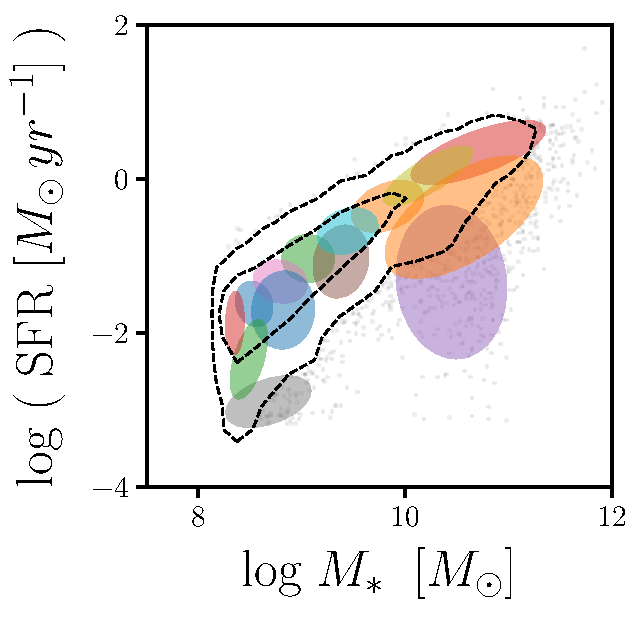
\includegraphics[width = 0.45\textwidth]{figs/SFRMstar_2Dgmm.pdf} 
\caption{Two-dimensional GMM fit to the SFR-$M_*$ relation of central galaxies
of the EAGLE simulation. The two-dimensional GMM fitting is an extension of the 
SFMS fitting method we describe in Section~\ref{sec:sfmsfit}. The colorful shaded
ellipses over-plotted on the SFR-$M_*$ relation (black) are the Gaussian components 
of the best-fit GMM. Although, identifying the SFMS from these Gaussian components
is difficult, the 2D GMM is effective in capturing the features of the SFR-$M_*$ 
relation and provides a good way comparing SFR-$M_*$ relations from different data.
} \label{fig:2dgmm}
\end{center}
\end{figure*}
%%%%%%%%%%%%%%%%%%%%%%%%%%%%%%%%%%%%%%%%%%

\section{Gaussian Mixture Models: 1D and Beyond}
In addition to identifying the SFMS, the GMM fitting method described above can 
be extended to describe the entire SFR-$M_*$ relation using a two-dimensional 
GMM. In Figure~\ref{fig:2dgmm}, we compare the instantaneous SFR to $M_*$ relation 
of central galaxies in the EAGLE simulation with the best-fit two-dimensional GMM. 
The over-plotted shaded ellipses represent the two-dimensional Gaussian components
of the best-fit GMM. Overall the best-fit 2D GMM captures the features in the 
EAGLE SFR-$M_*$ relation. It also provides a straightforward way of comparing 
different SFR-$M_*$ relations. However, as Figure~\ref{fig:2dgmm} illustrates, 
specifically identifying the SFMS using the two-dimensional model is more 
challenging. Therefore in this paper, we do not discuss the 2D GMM further. 


\section{Resolution Effects and Galaxies with $\mathrm{SFR} = 0$} \label{app:zerosfr}

%%%%%%%%%%%%%%%%%%%%%%%%%%%%%%%%%%%%%%%%%%
% Figure 
%%%%%%%%%%%%%%%%%%%%%%%%%%%%%%%%%%%%%%%%%%
\begin{figure*}
\begin{center}
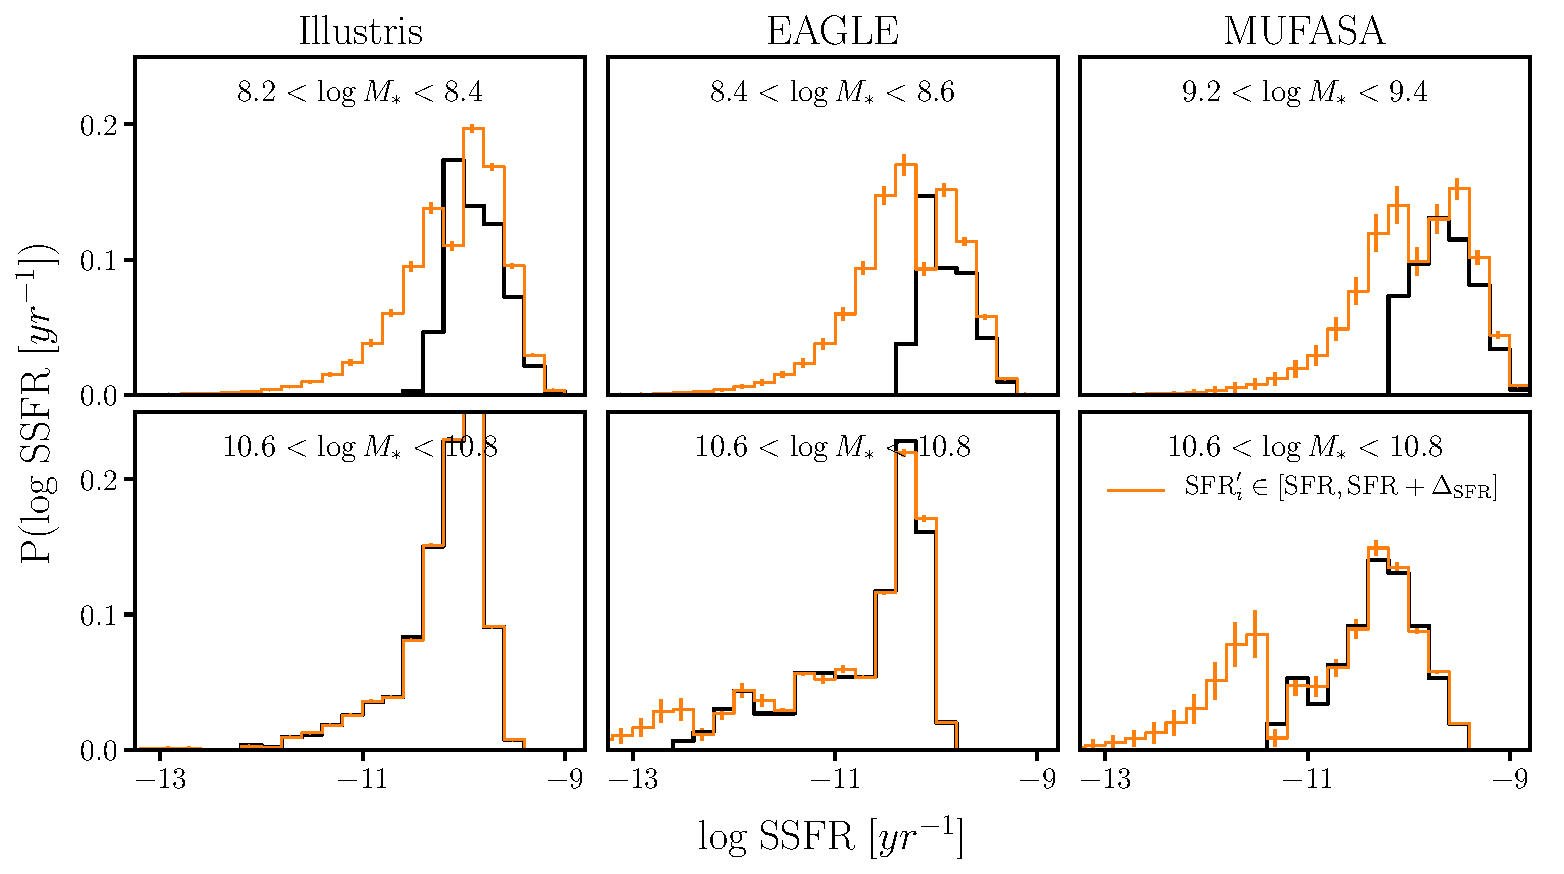
\includegraphics[width=0.9\textwidth]{figs/Pssfr_res_impact.pdf} 
\caption{The impact of SFR resolution and galaxies with SFR$=0$, on 
the SSFR distribution, $P(\mathrm{SSFR})$, of Illustris, EAGLE, and 
MUFSAS simulations. We plot $P(\mathrm{SSFR})$ with $\mathrm{SFR} = 0$
galaxies in blue and $P(\mathrm{SSFR})$ without $\mathrm{SFR} = 0$ 
galaxies in black. The uncertainties of $P(\mathrm{SSFR})$ is obtained 
from re-sampling the SFR of each galaxy based on the SFR resolution, 
as described in  Appendix~\ref{app:zerosfr}. For each simulation, we 
present two distinct stellar mass bins to illustrate the impact at low 
and high $M_*$.
} 
\label{fig:zerosfr_res}
\end{center}
\end{figure*}
%%%%%%%%%%%%%%%%%%%%%%%%%%%%%%%%%%%%%%%%%%

%%%%%%%%%%%%%%%%%%%%%%%%%%%%%%%%%%%%%%%%%%
% Figure 
%%%%%%%%%%%%%%%%%%%%%%%%%%%%%%%%%%%%%%%%%%
\begin{figure*}
\begin{center}
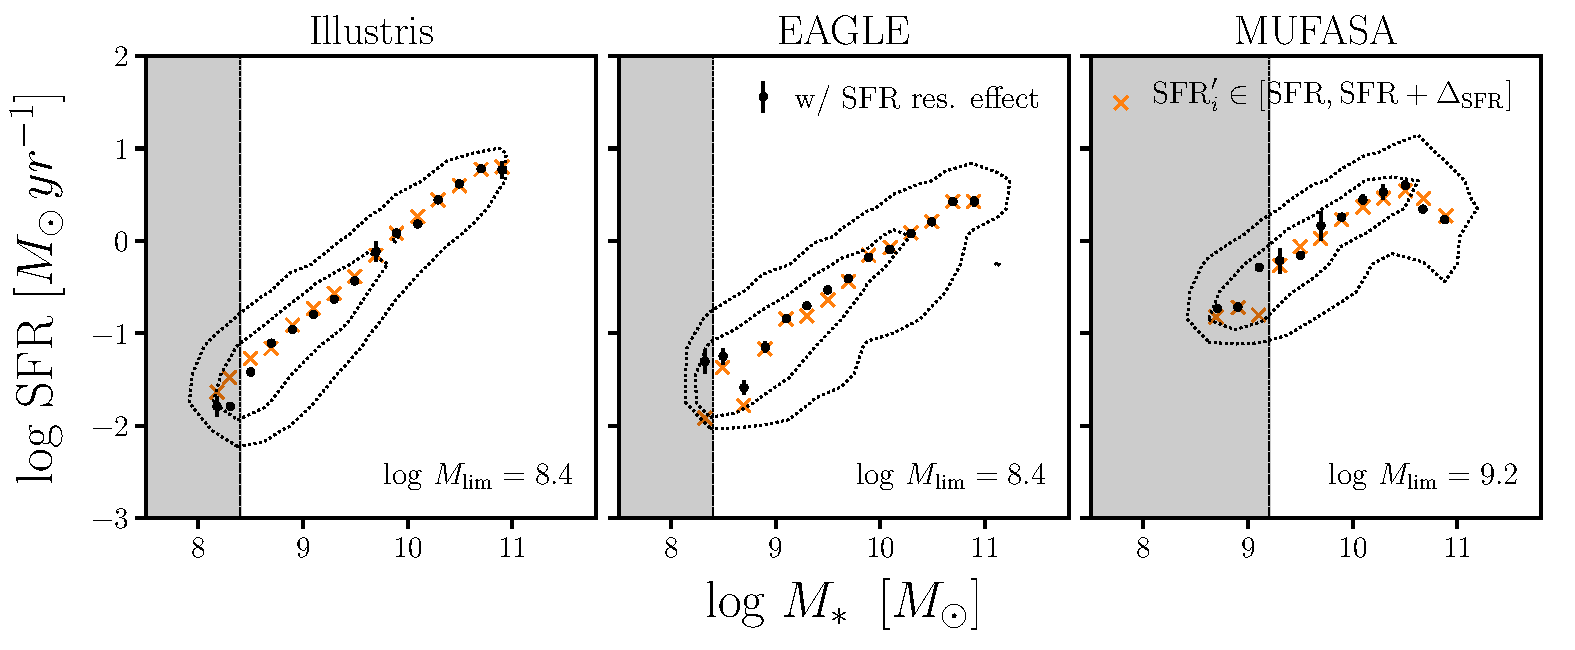
\includegraphics[width=0.8\textwidth]{figs/Mlim_res_impact.pdf} 
\caption{Resolution effects of hydrodynamical simulations (Illustris, 
EAGLE, and MUFASA) impact our SFMS fitting for SFR averaged over 
$100\,\mathrm{Myr}$ at low stellar mass. We therefore determine stellar
mass limits based on the discrepancy between the SFMS fits neglecting 
the resolution limit (black) and fits trying to include the resolution 
limit by re-sampling the SFRs (orange; Appendix~\ref{app:zerosfr}). For
Illustris, EAGLE, and MUFASA we set $\log M_\mathrm{lim} = 8.4, 8.6$, and 
$9.4$, respectively.} 
\label{fig:mlim_res}
\end{center}
\end{figure*}
%%%%%%%%%%%%%%%%%%%%%%%%%%%%%%%%%%%%%%%%%%

%%%%%%%%%%%%%%%%%%%%%%%%%%%%%%%%%%%%%%%%%%
% Figure 
%%%%%%%%%%%%%%%%%%%%%%%%%%%%%%%%%%%%%%%%%%
\begin{figure*}
\begin{center}
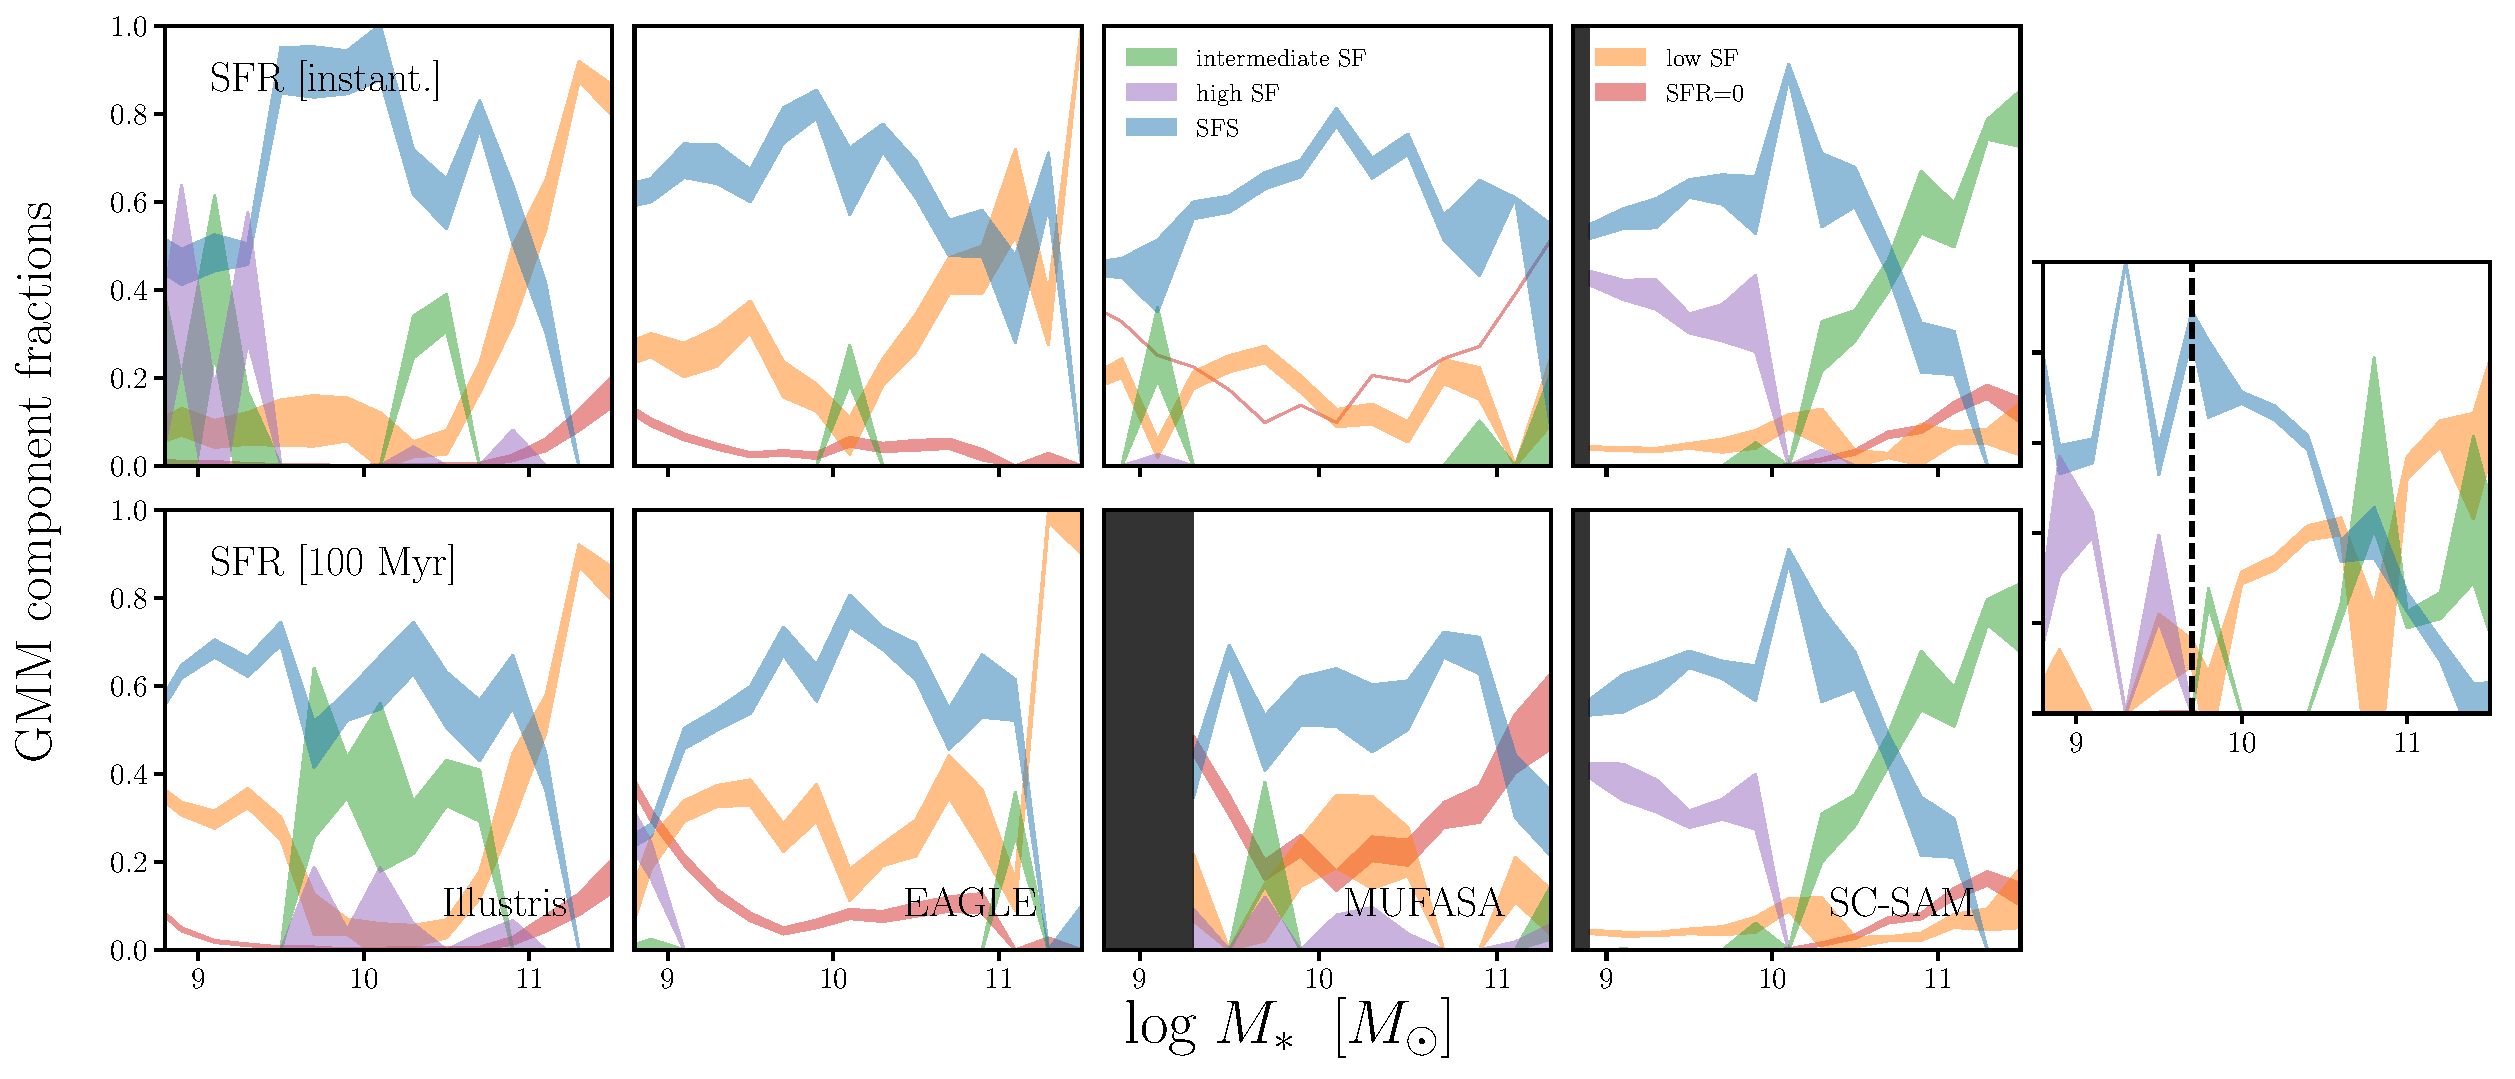
\includegraphics[width=0.9\textwidth]{figs/GMMcomp_comp_uncertainty.pdf} 
\caption{
} \label{fig:fcomp_uncertainty}
\end{center}
\end{figure*}
%%%%%%%%%%%%%%%%%%%%%%%%%%%%%%%%%%%%%%%%%%


\bibliographystyle{aasjournal}
\bibliography{paper1}
\end{document}